% (c) 2012 -2014 Dimitrios Vrettos - d.vrettos@gmail.com
% (c) 2014 Daniele Zambelli - daniele.zambelli@gmail.com

\input{\folder disequazioni_grafici}

\chapter{Disequazioni}

\section{Disuguaglianze chiuse e aperte}
\label{sec:dis_disguagianze}

Consideriamo le seguenti proposizioni:

\begin{enumeratea}
\item 5 è minore di~12;
\item \(48-90\) è maggiore di~30;
\item il quadrato di un numero reale è maggiore o uguale a zero;
\item sommando ad un numero la sua metà si ottiene un numero minore
o uguale a~1.
\end{enumeratea}

Esse possono essere tradotte in linguaggio matematico usando i simboli
\(>\) (maggiore), \(<\)~(minore), \({\geq}\) (maggiore o uguale), \({\leq}\) 
(minore o uguale) e precisamente:

\begin{multicols}{4}
 \begin{enumeratea}
\item \(5<12\)
\item \(48-90>30\)
\item \(x^{2}\ge~0\)
\item \(x+\dfrac{1}{2}x\le~1\).
 \end{enumeratea}
\end{multicols}

Le formule che contengono variabili si dicono aperte; quelle che
contengono solo numeri si dicono chiuse. Quindi a) e b) sono formule
chiuse; c) e d) sono formule aperte.

\begin{definizione}
Chiamiamo \emph{disuguaglianza} una formula chiusa
costruita con uno dei predicati:~\(<\) (essere minore);
\(>\) (essere maggiore); \({\leq}\) (essere minore o uguale);
\({\geq}\) (essere maggiore o uguale).
\end{definizione}

Di essa sappiamo subito stabilire il valore di verità, quando è
stabilito l'ambiente in cui vengono enunciate.

\begin{definizione}
Chiamiamo \emph{disequazione} una formula aperta,
definita in~\(\insR\) e costruita con uno dei seguenti predicati:~\(<\)
(essere minore); \(>\) (essere maggiore); \({\leq}\)
(essere minore o uguale); \({\geq}\) (essere
maggiore o uguale).
\end{definizione}

Analogamente a quanto detto per le equazioni, chiamiamo
\emph{incognite} le variabili che compaiono nella disequazione,
\emph{primo membro} e \emph{secondo membro} le due espressioni che
compaiono a sinistra e a destra del segno di disuguaglianza.

% \begin{exrig}
 \begin{esempio}
 Disuguaglianze vere e false.

 \begin{enumeratea}
\item in~\(\insN\), la formula~\(5>0\) è una disuguaglianza: vera;
\item in~\(\insZ\), la formula~\(-6>-4\) è una disuguaglianza: falsa;
\item la formula~\(5x>0\) è una disequazione; quando
all'incognita sostituiamo un numero essa si trasforma
in una disuguaglianza e solo allora possiamo stabilirne il valore di
verità. Nel caso proposto è vera se sostituiamo
alla variabile un qualunque numero positivo, falsa se
sostituiamo zero o un numero negativo.
\end{enumeratea}
 \end{esempio}

% \end{exrig}

% \ovalbox{\risolvi \ref{ese:21.8}}

\begin{definizione}
Chiamiamo \emph{Insieme Soluzione} (\(IS\)) di una disequazione, l'insieme 
dei valori che, sostituiti all'incognita, rendono vera la disuguaglianza.
\end{definizione}

Mentre le soluzioni di un'equazione determinata sono dei numeri isolati, 
le soluzioni delle disequazioni sono degli intervalli di numeri.
Ad esempio una disequazione può essere verificata da tutti i numeri positivi 
oppure da tutti i numeri compresi tra~\(-5\) e~\(+4,5\).

I numeri li conosciamo bene, sappiamo come rappresentarli, gli intervalli
un po' meno.
Prima di affrontare il nuovo argomento, vediamo dunque come rappresentare gli 
intervalli.

\section{Intervalli sulla retta}
\label{sec:dis_intervalli}

I \emph{numeri} possono essere rappresentati come \emph{punti} di una retta: 
ogni numero ha per immagine un punto della retta e viceversa ogni punto della 
retta è immagine di un numero. 
Un \emph{intervallo} di numeri può essere messo in corrispondenza con una 
\emph{semiretta} o un \emph{segmento}.
\begin{multicols}{2}
Un \emph{segmento} della retta \\
è l'insieme di \emph{tutti i punti compresi} tra due punti detti 
\emph{estremi} del segmento. 
\begin{center}
\disegno{\inticonasse{0}{-1.5}{+1.5}{-7}{+2}{blue}{blue}{x}}
\end{center}

Un \emph{intervallo} numerico \\
è l'insieme di \emph{tutti i numeri compresi} tra due numeri 
detti \emph{estremi} dell'intervallo. 

\vspace{1em}
\hspace{20mm} \(\quadra{-7;~+2}\)
% \vspace{-1.5em}
% \begin{center}
% \(\intervcc{-7}{+2}\)
% \end{center}
\end{multicols}

\osservazione Quando rappresentiamo un intervallo poniamo attenzione di 
scrivere prima il numero minore poi il maggiore.

``Tutti i numeri compresi tra~\(-7\) e~\(-2\)'' è una frase ambigua. 
È chiaro che:~\(-5;~-4;~-3; \dots\), ma anche:~\(-5,2;~-4,37;~-2,001; \dots\)  
appartengono all'intervallo, ma cosa dire di~\(-7\) e di~\(-2\)? A seconda dei 
gusti possiamo sostenere che gli estremi appartengono oppure no all'intervallo, 
non c'è una ragione logica per preferire una o l'altra interpretazione. 
Quindi i matematici parlano di due tipi di intervalli: 

\begin{itemize} [noitemsep]
 \item Intervalli \emph{chiusi}: quelli che comprendono anche gli estremi;
 \item Intervalli \emph{aperti}: quelli che non comprendono gli estremi.
\end{itemize}

Possiamo distinguere gli intervalli anche in base ad un'altra caratteristica:

\begin{itemize} [noitemsep]
 \item Intervalli \emph{limitati}: formati dai numeri compresi tra due numeri;
 \item Intervalli \emph{illimitati}: formati dai numeri minori (o maggiori) di
  un dato numero.
\end{itemize}

% Possiamo dare la seguente definizione:
% 
% \begin{definizione}
%  Si chiama \emph{intervallo} di un insieme ordinato, 
%  un sottoinsieme che contiene tutti gli elementi compresi tra due 
%  valori detti \emph{estremi}. 
%  Questi valori possono appartenere oppure non appartenere all'intervallo. 
% \end{definizione}

La situazione non è semplice, perché in un intervallo potrebbe essere 
compreso un estremo e non l'altro quindi possiamo avere intervalli 
aperti/chiusi a destra o a sinistra. 
Non solo, ma un intervallo potrebbe avere un inizio e poi continuare 
all'infinito vedi~\ref{tab:intervalli}.

\begin{table}[h!]
\caption{Intervalli}
\center
\label{tab:intervalli}
  \centering\begin{tabular}{>{\centering\arraybackslash}m{35mm}|
                            >{\centering\arraybackslash}m{25mm}|
                            >{\centering\arraybackslash}m{30mm}|
                            >{\centering\arraybackslash}m{35mm}} 
%  \begin{tabular}{p{4cm}|c|c|c}
  a parole   & con i predicati & con le parentesi & sulla retta \\
  \hline
  i numeri compresi tra \(a\) e~\(b\) estremi esclusi & 
  \(a < x < b\) & \((a;~b)\) o \(]a;~b[\) & 
  \disegno{\inticonasse{0}{-1.5}{+1.5}{a}{b}{white}{white}
  x}\\
  \hline
  i numeri compresi tra \(a\) e~\(b\) estremi inclusi & 
  \(a \le x \le b\) & \([a;~b]\) &  
  \disegno{\inticonasse{0}{-1.5}{+1.5}{a}{b}{blue}{blue}{x}} \\
  \hline
  i numeri compresi tra \(a\) e~\(b\), a~incluso, b~escluso & 
  \(a \le x < b\) & \([a;~b)\) o \([a;~b[\) &  
  \disegno{\inticonasse{0}{-1.5}{+1.5}{a}{b}{blue}{white}{x}} \\
  \hline
  i numeri compresi tra \(a\) e~\(b\), a~escluso, b~incluso & 
  \(a < x \le b\) & \((a;~b]\) o \(]a;~b]\) &  
  \disegno{\inticonasse{0}{-1.5}{+1.5}{a}{b}{white}{blue}{x}} \\
  \hline
  i numeri fino ad \(a\), \(a\)~escluso & 
  \(x < a\) & \((-\infty;~a)\) o \(]-\infty;~a[\) & 
  \disegno{\raylconasse{0}{5}{2.5}{a}{white}{x}} \\
  \hline
  i numeri fino ad \(a\), \(a\)~incluso & 
  \(x \le a\) & \((-\infty;~a]\) o \(]-\infty;~a]\) &  
  \disegno{\raylconasse{0}{5}{2.5}{a}{blue}{x}} \\
  \hline
  i numeri da \(a\) in poi, \(a\)~escluso & 
  \(x > a\) o \(a < x\) & \((a;~-\infty)\) o \(]a;~-\infty[\) & 
  \disegno{\rayrconasse{0}{5}{2.5}{a}{white}{x}} \\
  \hline
  i numeri da \(a\) in poi, \(a\)~incluso & 
  \(x \ge a\) o \(a \le x\) & \([a;~-\infty)\) o \([a;~-\infty[\) & 
  \disegno{\rayrconasse{0}{5}{2.5}{a}{blue}{x}} \\
  \hline
 \end{tabular}
\end{table}

% \begin{exrig}
\begin{esempio}
\(H=\{x\in \insR/x<3\}\) intervallo illimitato 
inferiormente~\(H = ]-\infty;~3) = (-\infty;~3)\).

L'insieme~\(H\) è rappresentato da tutti i punti della
semiretta che precede il punto~3, con 3 escluso. 
Nella retta evidenziamo questi punti e, per indicare che l'origine della 
semiretta non appartiene all'insieme abbiamo usato un pallino vuoto.
\vspace{-.5em}
\begin{center}
 \disegno{\raylconasse{0}{10}{5}{3}{white}{x}}
\end{center}
\end{esempio}

\begin{esempio}
\(\insP=\{x\in \insR/x\ge -5\}\) intervallo illimitato superiormente chiuso 
a sinistra~\(\insP = [-5;~+\infty[ = [-5;~+\infty)\).

Segniamo sulla retta~\(r\) il punto immagine di~\(-5\)
l'insieme~\(\insP\) è rappresentato dalla semiretta di tutti
i punti che seguono~\(-5\), compreso lo stesso~\(-5\). Nel disegno, la
semiretta dei punti che appartengono a~\(\insP\) è stata disegnata con una
linea più spessa, per indicare che il punto~\(-5\) appartiene
all'intervallo abbiamo messo un pallino pieno sul punto.
\vspace{-.5em}
\begin{center}
 \disegno{\rayrconasse{0}{10}{5}{-5}{blue}{x}}
\end{center}
\end{esempio}

\begin{esempio}
 \(D=\{x\in \insR/-2<x<6\}\) intervallo limitato 
 aperto~\(D = ]-2;~6[ = (-2;~6)\).

Segniamo sulla retta reale i punti immagine degli estremi del segmento,
\(-2\) e~6. L'insieme~\(D\) è rappresentato dal segmento che
ha per estremi questi due punti. Nel disegno il segmento è stato
disegnato con una linea più spessa, i due estremi del segmento sono
esclusi, pertanto su ciascuno di essi abbiamo messo un pallino vuoto.
\vspace{-.5em}
\begin{center}
 \disegno{\inticonasse{0}{0}{8}{-2}{6}{white}{white}{x}}
\end{center}
\end{esempio}

\begin{esempio}
\(T=\{x\in \insR/-2<x\le~6\}\) intervallo limitato chiuso a 
destra~\(T = ]-2;~6] = (-2;~6]\).

Rispetto al caso precedente, il segmento che rappresenta
l'insieme~\(T\) è chiuso a destra, ossia è incluso
nell'intervallo anche il~6, è escluso invece il
punto~\(-2\).
\vspace{-.5em}
\begin{center}
 \disegno{\inticonasse{0}{0}{8}{-2}{6}{white}{blue}{x}}
\end{center}
\end{esempio}

\begin{esempio}
\(S=\{x\in \insR/-2\le x\le~6\}\) intervallo chiuso e 
limitato~\(S = [2;~6]\).

Il segmento che rappresenta l'insieme~\(S\) contiene tutti e
due i suoi estremi:
\vspace{-.5em}
\begin{center}
 \disegno{\inticonasse{0}{0}{8}{-2}{6}{blue}{blue}{x}}
\end{center}
\end{esempio}

\begin{esempio}
Due particolari sottoinsiemi dei numeri reali sono:

\begin{itemize} [noitemsep]
\item \(\insR^{+}=\{x\in \insR/x>0\} = ]0;~\infty[\) \hspace{15mm}
\raisebox{-9pt}[0pt][0pt]{\disegno{\rayrconasse{0}{5}{2.5}{0}{white}{x}}} 
\item \(\insR^{-}=\{x\in \insR/x<0\} = ]- \infty;~0[\) \hspace{11mm}
\raisebox{-9pt}[0pt][0pt]{\disegno{\raylconasse{0}{5}{2.5}{0}{white}{x}}} 
\end{itemize}
\end{esempio}
% \end{exrig}

% \ovalbox{\risolvii \ref{ese:21.1}, \ref{ese:21.2}, \ref{ese:21.3}, 
% \ref{ese:21.4}, \ref{ese:21.5}, \ref{ese:21.6}, \ref{ese:21.7}}

\section{Segno di una funzione lineare}
\label{sec:dis_binomio}

% Prima di affrontare lo studio delle disequazioni è importante capire come 
% studiare il segno di un'espressione contenente una variabile. 
% In questo modo, le disequazioni si ridurranno ad una applicazione dello 
% studio del segno.
Studiare il segno di un'espressione che contiene la variabile~\(x\), vuol 
dire stabilire per quali valori della variabile l'espressione è negativa, per 
quali è nulla  e per quali è positiva.
Come esempio possiamo studiare i valori che assumono i due 
binomi~\(f(x) = -4 x +4\) e~\(g(x) = \dfrac{3}{2} x +3\) al variare di~\(x\).

Per farlo costruiamo una tabella con alcuni valori e disegniamo il grafico 
delle rette: \quad \(y=f(x)\) e \(y=g(x)\).

\begin{inaccessibleblock}[Figura: TODO]
 \begin{figure}[h]
 \begin{minipage}[]{.45\textwidth}
%   \centering% (c) 2014 Daniele Zambelli - daniele.zambelli@gmail.com

%%%
% Retta per due punti
%%%%
 
\begin{tikzpicture}[x=5mm, y=5mm, smooth]

\clip (-5.5, -5.5) rectangle (5.5, 5.9);

% (c) 2014 Daniele Zambelli - daniele.zambelli@gmail.com

%%%
% Piano cartesiano: da -5 a +5 scala 0,5
%%%%
% \usepgflibrary{arrows.meta}

% Griglia
\draw[gray!50, very thin, step=1] (-5.2, -5.2) grid (5.2, 5.2);

%Asse x
\draw [-{Stealth[length=2mm, open, round]}] (-5.3,0) -- (5.5,0) node [below]  {$x$};

%Asse y
\draw [-{Stealth[length=2mm, open, round]}] (0, -5.3) -- (0, 5.5) node [left]  {$y$};

\node [below] at (-.3, 0) {O};


\coordinate (inizio) at (-1, 8);
\coordinate (zero) at (1, 0);
\coordinate (fine) at (3, -8);

\draw [-] [ultra thick,blue!50!black] (inizio) -- (zero);
\draw [-] [ultra thick,red!50!black] (zero) -- (fine);

\end{tikzpicture}

\begin{center}
 \begin{tabular}{c|c|c}
  \(x\) & \(f(x) = -4 x +4\) & \(g(x) = \dfrac{3}{2} x +6\) \\
  \hline
  \(-4\) & \(+20\) & \(-3\) \\
  \(-3\) & \(+16\) & \(-1,5\) \\
  \(-2\) & \(+12\) & \(0\) \\
  \(-1\) & \(+8\) & \(+1,5\) \\
  \( 0\) & \(+4\) & \(+3\) \\
  \( 1\) & \(0\) & \(+4,5\) \\
  \( 2\) & \(-4\) & \(+6\) \\
  \( 3\) & \(-8\) & \(+7,5\) %\\
%   \( 4\) & \(-12\) & \(+9\) \\
%   \( 5\) & \(-16\) & \(+21\)
 \end{tabular}
\end{center}
 \end{minipage}
 \hfill
 \begin{minipage}[]{.25\textwidth}
%   \centering% (c) 2014 Daniele Zambelli - daniele.zambelli@gmail.com

%%%
% Retta per due punti
%%%%
 
\begin{tikzpicture}[x=5mm, y=5mm, smooth]

\clip (-5.5, -5.5) rectangle (5.5, 5.9);

% (c) 2014 Daniele Zambelli - daniele.zambelli@gmail.com

%%%
% Piano cartesiano: da -5 a +5 scala 0,5
%%%%
% \usepgflibrary{arrows.meta}

% Griglia
\draw[gray!50, very thin, step=1] (-5.2, -5.2) grid (5.2, 5.2);

%Asse x
\draw [-{Stealth[length=2mm, open, round]}] (-5.3,0) -- (5.5,0) node [below]  {$x$};

%Asse y
\draw [-{Stealth[length=2mm, open, round]}] (0, -5.3) -- (0, 5.5) node [left]  {$y$};

\node [below] at (-.3, 0) {O};


\coordinate (inizio) at (-1, 8);
\coordinate (zero) at (1, 0);
\coordinate (fine) at (3, -8);

\draw [-] [ultra thick,blue!50!black] (inizio) -- (zero);
\draw [-] [ultra thick,red!50!black] (zero) -- (fine);

\end{tikzpicture}

\begin{center} 
\disrettaa 
\vspace{3mm}
\(y = -4 x +4\)
\end{center}
 \end{minipage}
 \hfill
 \begin{minipage}[]{.25\textwidth}
%   \centering% (c) 2014 Daniele Zambelli - daniele.zambelli@gmail.com

%%%
% Retta per due punti
%%%%
 
\begin{tikzpicture}[x=5mm, y=5mm, smooth]

\clip (-5.5, -5.5) rectangle (5.5, 5.9);

% (c) 2014 Daniele Zambelli - daniele.zambelli@gmail.com

%%%
% Piano cartesiano: da -5 a +5 scala 0,5
%%%%
% \usepgflibrary{arrows.meta}

% Griglia
\draw[gray!50, very thin, step=1] (-5.2, -5.2) grid (5.2, 5.2);

%Asse x
\draw [-{Stealth[length=2mm, open, round]}] (-5.3,0) -- (5.5,0) node [below]  {$x$};

%Asse y
\draw [-{Stealth[length=2mm, open, round]}] (0, -5.3) -- (0, 5.5) node [left]  {$y$};

\node [below] at (-.3, 0) {O};


\coordinate (inizio) at (-6, -6);
\coordinate (zero) at (-2, 0);
\coordinate (fine) at (2, 6);

\draw [-] [ultra thick,red!50!black] (inizio) -- (zero);
\draw [-] [ultra thick,blue!50!black] (zero) -- (fine);

\end{tikzpicture}

\begin{center} 
\disrettab 
\(y = \dfrac{3}{2} x +3\)
\end{center}
 \end{minipage}
\end{figure}
\end{inaccessibleblock}

Si può osservare che il primo binomio è sempre positivo finché~\(x\) è più 
piccolo di~1, quando~\(x\) vale proprio 1 il binomio vale~0, quando~\(x\) è 
maggiore di~1 il binomio assume un valore negativo.
Il secondo binomio ha un comportamento diverso. Finché~\(x\) si mantiene 
minore di~\(-2\) è negativo, quando~\(x\) vale~\(-2\) il binomio vale~0, 
quando~\(x\) supera il valore~\(-2\) il binomio diventa positivo.

In realtà noi abbiamo verificato solo un piccolissimo insieme di valori, 
ma l'andamento regolare dei risultati dovrebbe convincerci che i segni 
rimangono immutati anche per valori molto diversi da quelli testati.

I grafici delle funzioni \(y=f(x)\) e \(y=g(x)\) sono due rette. 
In corrispondenza dei valori positivi del polinomio, le rette si trovano al 
di sopra dell'asse~\(x\)% (tratto blu)
, quando invece il polinomio assume valori negativi, le rette si trovano 
sotto all'asse~\(x\)% (tratto rosso)
.

Disegnare una retta nel piano cartesiano è un'abilità molto utile da 
possedere, ma per il nostro problema si può tracciare il grafico in modo 
molto approssimato: sono due gli aspetti che dobbiamo riportare nel grafico:

\begin{enumerate} [noitemsep]
 \item 
  lo zero del polinomio, cioè il punto in cui la retta interseca 
  l'asse~\(x\);
 \item
  l'andamento della retta: cioè se la retta è crescente o decrescente.
\end{enumerate}

Si capisce facilmente se la retta è crescente o decrescente guardando la sua 
equazione infatti le rette \emph{crescenti} hanno il coefficiente della~\(x\) 
\emph{positivo}, mentre le rette \emph{decrescenti} hanno il coefficiente 
della~\(x\) \emph{negativo}.
Quindi i grafici possono essere tracciati semplicemente in questo modo:

\begin{inaccessibleblock}[Figura: TODO]
 \begin{figure}[h]
 \centering
 \begin{minipage}[]{.45\textwidth}
  \centering\rettadec{+1}
  \caption{Retta~\(y = f(x) = -4 x +4\)}
 \end{minipage}
 \begin{minipage}[]{.45\textwidth}
  \centering\rettacre{-2}
  \caption{Retta~\(y = g(x) = \frac{3}{2} x +3\)}
 \end{minipage}
\end{figure}
\end{inaccessibleblock}

Su questi ultimi grafici si possono aggiungere le informazioni che 
interessano lo studio del segno:

\begin{itemize} [noitemsep]
 \item il valore della~\(x\) che rende uguale a 0 il polinomio;
 \item l'intervallo dell'asse~\(x\) per il quale il polinomio è positivo;
 \item l'intervallo dell'asse~\(x\) per il quale il polinomio è negativo.
\end{itemize}

\begin{inaccessibleblock}[Figura: TODO]
 \begin{figure}[h]
 \centering
 \begin{minipage}[]{.45\textwidth}
  \centering\segnidec{+1}
  \caption{Segno di~\(y = f(x) = -4 x +4\)}
 \end{minipage}
 \begin{minipage}[]{.45\textwidth}
  \centering\segnicre{-2}
  \caption{Segno di~\(y = g(x) = \frac{3}{2} x +3\)}
 \end{minipage}
\end{figure}
\end{inaccessibleblock}

Riassumendo, per studiare il segno di un binomio di primo grado dobbiamo: 

\begin{procedura}
 Studio del segno di un binomio di primo grado:
\begin{enumeratea}
\item calcolare lo zero del polinomio risolvendo un'equazione associata al 
 polinomio;
\item disegnare il grafico della funzione associata al polinomio, 
 tenendo conto se la retta è crescente o decrescente.
\item riportare su questo grafico lo zero del polinomio e segnare con un 
 "+" i tratti positivi (quelli sopra l'asse delle~\(x\)) e con un "-" i 
 tratti  negativi (quelli nei quali la retta è tracciata sotto l'asse 
delle~\(x\)).
\end{enumeratea}
\end{procedura}

Riassumendo, lo studio del segno del binomio di primo 
grado:~\(f(x) = -4 x +4\), si riduce a svolgere questi due passi:

\begin{enumerate}
 \item
  Equazione Associata:~\(-4 x +4 = 0 \quad \Rightarrow \quad x = 1\)
 \item 
  \begin{minipage}{.45\textwidth}
  Funzione Associata: \(y = -4 x +4 \quad \rightarrow\)
  \end{minipage}
  \begin{minipage}{.30\textwidth}
  \segnidec{+1}
  \end{minipage}
\end{enumerate}

\section{Segno di un prodotto}
\label{sec:dis_prodotto}

Imparato come studiare il segno di un binomio di primo grado possiamo 
incominciare a complicare le cose\dots
Se dobbiamo studiare il segno del prodotto tra polinomi, possiamo 
seguire un procedimento formato da questi 2 passi:

\begin{procedura}
 Studio del segno del prodotto di polinomi:
\begin{enumeratea}
\item studiare il segno di ogni singolo fattore;
\item applicare la regola dei segni.
\end{enumeratea}
\end{procedura}

Per quanto riguarda il primo punto seguiamo le indicazioni precedenti. 

Il secondo lo si risolve con un grafo con
\begin{itemize} [noitemsep]
\item tanti assi~\(x\) quanti sono i fattori, 
\item tante linee verticali quanti sono i diversi zeri dei polinomi. 
\end{itemize}

Intestiamo ogni riga verticale con il valore di uno zero del polinomio
stando ben attenti di riportarli in \emph{ordine crescente} e intestiamo ogni 
\emph{spazio orizzontale} con l'indicazione del fattore di cui vogliamo 
riportare il segno. 

Preparato questo schema, tracciamo un tondino in corrispondenza degli zeri 
dei polinomi e riportiamo i segni già studiati precedentemente. 

Sopra al terzo asse~\(x\) riportiamo il segno del prodotto ottenuto 
seguendo la solita regola: 
\begin{itemize} [noitemsep]
\item è \emph{negativo} se i fattori negativi sono in numero dispari, 
\item è \emph{nullo} se almeno un fattore è nullo.
\item un prodotto è \emph{positivo} se i fattori negativi sono in numero 
pari, 
\end{itemize}

% \begin{exrig}
\begin{esempio}
Applichiamo questo procedimento allo studio del segno del 
prodotto: \\
\(f(x)=(x-4)(x+2)\).

Chiamiamo \(f_1(x)=\tonda{x-4}\) \quad e \quad \(f_2(x)=\tonda{x+2}\)

\begin{itemize} [noitemsep]
 \item Studio del segno del primo fattore~\(f_1\):\\
 
\segnoretta{x - 4 = 0 \quad \Rightarrow \quad x = 4}
           {y = x - 4 \quad \rightarrow}
           {\segnicre{4}}
%  \begin{minipage}{.45\textwidth}
%   E.A.:~\(x - 4 = 0 \quad \Rightarrow \quad x = 4\)
%  \end{minipage}
%  \begin{minipage}{.25\textwidth}
%   F.A.:~\(y = x - 4 \quad \rightarrow\)
%  \end{minipage}
%  \begin{minipage}{.3\textwidth}
% %   % (c) 2014 Daniele Zambelli - daniele.zambelli@gmail.com

%%%
% Segno di un polinomio: crescente, zero=4.
%%%%
 
\begin{tikzpicture}[x=1.5mm, y=1.5mm, smooth]

% (c) 2014 Daniele Zambelli - daniele.zambelli@gmail.com

%%%
% Retta crescente con segni
%%%%
 
\coordinate (inizio) at (-10, -4);
\coordinate (zero) at (0, 0);
\coordinate (fine) at (10, 4);

% (c) 2014 Daniele Zambelli - daniele.zambelli@gmail.com

%%%
% Asse cartesiano x
%%%%

\input{lbr/assiepiani/asse10.pgf}
\node [below] at (10, 0)  {$x$};


\draw [-] [ultra thick, red!50!black] (inizio) -- (zero);
\draw [-] [ultra thick, blue!50!black] (zero) -- (fine);

\node [xshift=-25, yshift=-3, above] at (zero) {$-$};
\draw[blue, thick, fill=white] (zero) circle (2pt);
\node [xshift=25, yshift=-3, above] at (zero) {$+$};

\node [above] {$4$};

\end{tikzpicture}

%   \segnicre{4}
%  \end{minipage}
 \item Studio del segno del secondo fattore~\(f_2\):\\
 \begin{minipage}{.45\textwidth}
  E.A.:~\(x + 2 = 0 \quad \Rightarrow \quad x=-2\)
 \end{minipage}
 \begin{minipage}{.25\textwidth}
  F.A.:~\(y = x + 2 \quad \rightarrow\)
 \end{minipage}
 \begin{minipage}{.3\textwidth}
%   % (c) 2014 Daniele Zambelli - daniele.zambelli@gmail.com

%%%
% Segno di un polinomio: crescente, zero=-2.
%%%%
 
\begin{tikzpicture}[x=1.5mm, y=1.5mm, smooth]

% (c) 2014 Daniele Zambelli - daniele.zambelli@gmail.com

%%%
% Retta crescente con segni
%%%%
 
\coordinate (inizio) at (-10, -4);
\coordinate (zero) at (0, 0);
\coordinate (fine) at (10, 4);

% (c) 2014 Daniele Zambelli - daniele.zambelli@gmail.com

%%%
% Asse cartesiano x
%%%%

\input{lbr/assiepiani/asse10.pgf}
\node [below] at (10, 0)  {$x$};


\draw [-] [ultra thick, red!50!black] (inizio) -- (zero);
\draw [-] [ultra thick, blue!50!black] (zero) -- (fine);

\node [xshift=-25, yshift=-3, above] at (zero) {$-$};
\draw[blue, thick, fill=white] (zero) circle (2pt);
\node [xshift=25, yshift=-3, above] at (zero) {$+$};

\node [above] {$-2$};

\end{tikzpicture}

  \segnicre{-2}
 \end{minipage}
 \item Grafo dei segni:
 
 \segnoprodottoa
 
 Oppure, usando il nome dato ai fattori: 
 
 \segnoprodottoas
 \item Possiamo concludere che il prodotto 
 \(f(x) = f_1(x) \cdot f_2(x)=(x -4)(x +2)\) è:
\begin{itemize} [noitemsep]
\begin{minipage}{.4\textwidth}
 \item positivo per~\(x < -2\) o per~\(x > +4\)
 \item nullo per~\(x = -2\) o per~\(x = +4\)
 \item negativo per~\(x > -2\) e~\(x < +4\)
\end{minipage}
\hfill
\begin{minipage}{.48\textwidth}
\begin{center}
\emph{Che possiamo sintetizzare con l'espressione}:\\
\(++\quadra{-2}--\quadra{+4}++\)
\end{center}
\end{minipage}
\end{itemize}
\end{itemize}
\end{esempio}
% \end{exrig}

\section{Segno di un quoziente}
\label{sec:dis_quoziente}

Dato che la regola del segno del quoziente è uguale alla regola del 
segno del prodotto,
si può utilizzare un metodo simile a quello presentato sopra anche 
per studiare il segno del quoziente di funzioni.

C'è un'unica \emph{piccola differenza}: perché si possa calcolare una 
frazione, il suo denominatore deve essere \emph{diverso da zero} (la 
differenza è \emph{piccola} ma \emph{importante}). 
Quindi non sono mai accettabili i valori di \(x\) che rendono nullo il 
denominatore.
Per ricordarci di questo, nel grafo dei segni, indichiamo con una 
\emph{crocetta} invece che con un cerchietto gli zeri del denominatore.

\begin{esempio}
Applichiamo questo procedimento allo studio del segno del quoziente: \\
\(f(x)=\dfrac{-3x-4}{2x+7}\).

Chiamiamo \(num(x)=-3x-4\) \quad e \quad \(den(x)=2x+7\)

\begin{itemize} [noitemsep]
 \item Studio del segno del numeratore~\(num(x)\):\\
 \begin{minipage}{.45\textwidth}
  E.A.:~\(-3x-4 = 0 \quad \Rightarrow \quad x = -\dfrac{4}{3}\)
 \end{minipage}
 \begin{minipage}{.25\textwidth}
  F.A.:~\(y = -3x-4 \quad \rightarrow\)
 \end{minipage}
 \begin{minipage}{.3\textwidth}
  \segnidec{-\dfrac{4}{3}}
 \end{minipage}
 \item Studio del segno del denominatore~\(den(x)\):\\
 \begin{minipage}{.45\textwidth}
  E.A.:~\(2x+7 = 0 \quad \Rightarrow \quad x=-\dfrac{7}{2}\)
 \end{minipage}
 \begin{minipage}{.25\textwidth}
  F.A.:~\(y = 2x+7 \quad \rightarrow\)
 \end{minipage}
 \begin{minipage}{.3\textwidth}
  \segnicre{-\dfrac{7}{2}}
 \end{minipage}
 \item Grafo dei segni \(\tonda{-\frac{7}{2} < -\frac{4}{3}\quad 
 \text{ dato che} \quad -7 \cdot 3 < -4 \cdot 2}\):
 
 \segnoquozientea
 
 Oppure, usando il nome dato ai fattori: 
 
 \segnoquozienteas
 \item Possiamo concludere che il quoziente 
 \(f(x) = \dfrac{num(x)}{den(x)}=\dfrac{-3x-4}{2x+7}\) è:
\begin{itemize} [noitemsep]
\begin{minipage}{.4\textwidth}
 \item negativo per \(x\) minore di \(-\dfrac{7}{2}\) o maggiore 
 di \(-\dfrac{4}{3}\)
 \item nullo per \(x\) uguale a \(-\dfrac{4}{3}\)
 \item non definito per \(x\) uguale a \(-\dfrac{7}{2}\)
 \item positivo per \(x\) compreso tra \(-\dfrac{7}{2}\) e \(-\dfrac{4}{3}\)
%  \item negativo per~\(x < -\dfrac{7}{2}\)~o~\(x > -\dfrac{4}{3}\)
%  \item nullo per~\(x = -\dfrac{4}{3}\)
%  \item non è definito per~\(x = -\dfrac{7}{2}\)
%  \item positivo per~\(-\dfrac{7}{2} < x < -\dfrac{4}{3}\)
\end{minipage}
\hfill
\begin{minipage}{.48\textwidth}
\begin{center}
\emph{Che possiamo sintetizzare con l'espressione}:\\ [1em]
\(--\rquadra{-\dfrac{7}{2}}++\quadra{-\dfrac{4}{3}}--\)\\ [1em]
(Notare il verso delle parentesi quadre!)
\end{center}
\end{minipage}
\end{itemize}
\end{itemize}
\end{esempio}

\section{Combinazione dei metodi}
\label{sec:dis_quoziente}

% \begin{exrig}
 \begin{esempio}
Applichiamo questo procedimento allo studio del segno della frazione:

\[f(x)=\frac{x(1 -2 x)(1 + 2 x)}{(x -2)(x +5)}\]

Chiamiamo:~\(n_1\),~\(n_2\)~e~\(n_3\) i fattori che si trovano al numeratore 
e:~\(d_1\)~e~\(d_2\) i fattori che si trovano al denominatore.

\begin{itemize} [noitemsep]
 \item Studio del segno del fattore~\(n_1\):\\
 \begin{minipage}{.45\textwidth}
  E.A.:~\(x=0 \Rightarrow x=0\)
 \end{minipage}
 \begin{minipage}{.25\textwidth}
  F.A.:~\(y = x \quad \rightarrow\)
 \end{minipage}
 \begin{minipage}{.3\textwidth}
%   % (c) 2014 Daniele Zambelli - daniele.zambelli@gmail.com

%%%
% Retta crescente zero in 0
%%%%
 
\begin{tikzpicture}[x=1.5mm, y=1.5mm, smooth]

% (c) 2014 Daniele Zambelli - daniele.zambelli@gmail.com

%%%
% Retta crescente con segni
%%%%
 
\coordinate (inizio) at (-10, -4);
\coordinate (zero) at (0, 0);
\coordinate (fine) at (10, 4);

% (c) 2014 Daniele Zambelli - daniele.zambelli@gmail.com

%%%
% Asse cartesiano x
%%%%

\input{lbr/assiepiani/asse10.pgf}
\node [below] at (10, 0)  {$x$};


\draw [-] [ultra thick, red!50!black] (inizio) -- (zero);
\draw [-] [ultra thick, blue!50!black] (zero) -- (fine);

\node [xshift=-25, yshift=-3, above] at (zero) {$-$};
\draw[blue, thick, fill=white] (zero) circle (2pt);
\node [xshift=25, yshift=-3, above] at (zero) {$+$};

\node [above] (0, 0) {$0$};

\end{tikzpicture}

  \segnicre{0}
 \end{minipage}
 \item Studio del segno del fattore~\(n_2\):\\
 \begin{minipage}{.45\textwidth}
  E.A.:~\(-2 x +1=0 \Rightarrow x=\frac{1}{2}\)
 \end{minipage}
 \begin{minipage}{.25\textwidth}
  F.A.:~\(y = -2 x +1 \quad \rightarrow\)
 \end{minipage}
 \begin{minipage}{.3\textwidth}
%   % (c) 2014 Daniele Zambelli - daniele.zambelli@gmail.com

%%%
% Retta decrescente zero in 1/2
%%%%
 
\begin{tikzpicture}[x=1.5mm, y=1.5mm, smooth]

% (c) 2014 Daniele Zambelli - daniele.zambelli@gmail.com

%%%
% Retta decrescente con segni
%%%%
 
\coordinate (inizio) at (-10, 4);
\coordinate (zero) at (0, 0);
\coordinate (fine) at (10, -4);

% (c) 2014 Daniele Zambelli - daniele.zambelli@gmail.com

%%%
% Asse cartesiano x
%%%%

\input{lbr/assiepiani/asse10.pgf}
\node [below] at (10, 0)  {$x$};


\draw [-] [ultra thick, blue!50!black] (inizio) -- (zero);
\draw [-] [ultra thick, red!50!black] (zero) -- (fine);

\node [xshift=-25, yshift=-3, above] at (zero) {$+$};
\draw[blue, thick, fill=white] (zero) circle (2pt);
\node [xshift=25, yshift=-3, above] at (zero) {$-$};

\node [above] {$+\frac{1}{2}$};

\end{tikzpicture}

  \segnidec{\frac{1}{2}}
 \end{minipage}
 \item Studio del segno del fattore~\(n_3\):\\
 \begin{minipage}{.45\textwidth}
  E.A.:~\(2 x +1=0 \Rightarrow x=- \frac{1}{2}\)
 \end{minipage}
 \begin{minipage}{.25\textwidth}
  F.A.:~\(y=2 x +1 \quad \rightarrow\)
 \end{minipage}
 \begin{minipage}{.3\textwidth}
%   % (c) 2014 Daniele Zambelli - daniele.zambelli@gmail.com

%%%
% Retta crescente zero in -1/2
%%%%
 
\begin{tikzpicture}[x=1.5mm, y=1.5mm, smooth]

% (c) 2014 Daniele Zambelli - daniele.zambelli@gmail.com

%%%
% Retta crescente con segni
%%%%
 
\coordinate (inizio) at (-10, -4);
\coordinate (zero) at (0, 0);
\coordinate (fine) at (10, 4);

% (c) 2014 Daniele Zambelli - daniele.zambelli@gmail.com

%%%
% Asse cartesiano x
%%%%

\input{lbr/assiepiani/asse10.pgf}
\node [below] at (10, 0)  {$x$};


\draw [-] [ultra thick, red!50!black] (inizio) -- (zero);
\draw [-] [ultra thick, blue!50!black] (zero) -- (fine);

\node [xshift=-25, yshift=-3, above] at (zero) {$-$};
\draw[blue, thick, fill=white] (zero) circle (2pt);
\node [xshift=25, yshift=-3, above] at (zero) {$+$};

\node [above] {$-\frac{1}{2}$};

\end{tikzpicture}

  \segnicre{-\frac{1}{2}}
 \end{minipage}
 \item Studio del segno del fattore~\(d_1\):\\
 \begin{minipage}{.45\textwidth}
  E.A.:~\(x-2=0 \Rightarrow x=2\)
 \end{minipage}
 \begin{minipage}{.25\textwidth}
  F.A.:~\(y=x-2 \quad \rightarrow\)
 \end{minipage}
 \begin{minipage}{.3\textwidth}
%   % (c) 2014 Daniele Zambelli - daniele.zambelli@gmail.com

%%%
% Retta crescente zero in 2
%%%%
 
\begin{tikzpicture}[x=1.5mm, y=1.5mm, smooth]

% (c) 2014 Daniele Zambelli - daniele.zambelli@gmail.com

%%%
% Retta crescente con segni
%%%%
 
\coordinate (inizio) at (-10, -4);
\coordinate (zero) at (0, 0);
\coordinate (fine) at (10, 4);

% (c) 2014 Daniele Zambelli - daniele.zambelli@gmail.com

%%%
% Asse cartesiano x
%%%%

\input{lbr/assiepiani/asse10.pgf}
\node [below] at (10, 0)  {$x$};


\draw [-] [ultra thick, red!50!black] (inizio) -- (zero);
\draw [-] [ultra thick, blue!50!black] (zero) -- (fine);

\node [xshift=-25, yshift=-3, above] at (zero) {$-$};
\draw[blue, thick, fill=white] (zero) circle (2pt);
\node [xshift=25, yshift=-3, above] at (zero) {$+$};

\node [above] {$+2$};

\end{tikzpicture}

  \segnicre{+2}
 \end{minipage}
 \item Studio del segno del fattore~\(d_2\):\\
 \begin{minipage}{.45\textwidth}
  E.A.:~\(x+5=0 \Rightarrow x=-5\)
 \end{minipage}
 \begin{minipage}{.25\textwidth}
  F.A.:~\(y=x+5 \quad \rightarrow\)
 \end{minipage}
 \begin{minipage}{.3\textwidth}
%   % (c) 2014 Daniele Zambelli - daniele.zambelli@gmail.com

%%%
% Retta crescente zero in -5
%%%%
 
\begin{tikzpicture}[x=1.5mm, y=1.5mm, smooth]

% (c) 2014 Daniele Zambelli - daniele.zambelli@gmail.com

%%%
% Retta crescente con segni
%%%%
 
\coordinate (inizio) at (-10, -4);
\coordinate (zero) at (0, 0);
\coordinate (fine) at (10, 4);

% (c) 2014 Daniele Zambelli - daniele.zambelli@gmail.com

%%%
% Asse cartesiano x
%%%%

\input{lbr/assiepiani/asse10.pgf}
\node [below] at (10, 0)  {$x$};


\draw [-] [ultra thick, red!50!black] (inizio) -- (zero);
\draw [-] [ultra thick, blue!50!black] (zero) -- (fine);

\node [xshift=-25, yshift=-3, above] at (zero) {$-$};
\draw[blue, thick, fill=white] (zero) circle (2pt);
\node [xshift=25, yshift=-3, above] at (zero) {$+$};

\node [above] {$-5$};

\end{tikzpicture}

  \segnicre{+5}
 \end{minipage}
 \item Applichiamo la regola dei segni ricordandoci di segnare con una 
 \disegno{\crocetta{0}{0}} %``X''
  gli zeri del denominatore:

  \segnomista
 \item Possiamo concludere che la funzione
 \(f(x)=\dfrac{x(1 -2 x)(1 + 2 x)}{(x -2)(x +5)}\) è:
\begin{itemize} [noitemsep]
 \item positiva per tutti i valori di~\(x\) minori di~\(-5\)
 \item non definita per~\(x=-5\)
 \item negativa per tutti i valori di~\(x\) compresi tra~\(-5\) e~\(-\frac{1}{2}\)
 \item zero per~\(x=-\frac{1}{2}\)
 \item positiva per tutti i valori di~\(x\) compresi tra~\(-\frac{1}{2}\) e~\(0\)
 \item zero per~\(x=0\)
 \item negativa per tutti i valori di~\(x\) compresi tra~\(0\) e~\(\frac{1}{2}\)
 \item zero per~\(x=\frac{1}{2}\)
 \item positiva per tutti i valori di~\(x\) compresi tra~\(\frac{1}{2}\) e~\(2\)
 \item non definita per~\(x=2\)
 \item negativa per tutti i valori di~\(x\) maggiori di~\(2\).
\end{itemize}
\end{itemize}
 \end{esempio}
% \end{exrig}

O in simboli:

\(x \in \mathbb{R} - \{ -5;~2 \}\) (insieme di esistenza)

\(\begin{array}{cccccccccc}
f(x) & > & 0 & \Leftrightarrow &
 x < -5 & \lor & -\frac{1}{2} < x < 0 & \lor & \frac{1}{2} < x < 2 \\
f(x) & = & 0 & \Leftrightarrow &
 x = -\frac{1}{2} & \lor & x = 0 & \lor & x = \frac{1}{2} \\
f(x) & < & 0 & \Leftrightarrow &
 -5 < x < -\frac{1}{2} & \lor & 0 < x < \frac{1}{2} & \lor & x > 2 \\
\end{array}\)

\vspace{1em}
O con un'espressione:
\[++\rquadra{-5}--\quadra{-\dfrac{1}{2}}++\quadra{0}
  --\quadra{+\dfrac{1}{2}}--\rquadra{+2}--\]

\section{Disequazioni numeriche}
\label{sec:dis_numeriche}

\subsection{Principi di equivalenza delle disequazioni}

Per lavorare sulle disequazioni si ricorre a due principi, che derivano 
direttamente dalle proprietà delle disuguaglianze.

Stabiliamo innanzitutto la seguente definizione:

\begin{definizione}
Due disequazioni si dicono \emph{equivalenti} se hanno lo
stesso insieme soluzione.
\end{definizione}

Stabilito questo, possiamo formulare due principi di equivalenza
simili a quelli validi per le equazioni

\begin{principio}[I principio]
\label{ppd}
Addizionando o sottraendo a ciascuno dei due membri di
una disequazione una stessa espressione (definita per qualunque
valore attribuito all'incognita), si ottiene una
disequazione equivalente alla data.
\end{principio}

Regola pratica: questo principio ci permette di
\begin{itemize} [nosep]
\item ``eliminare'' da entrambi i membri gli addendi uguali;
\item ``spostare'' a primo membro tutti i termini, lasciando nel secondo il 
numero zero.
\end{itemize}

\begin{principio}[II principio]
Moltiplicando o dividendo ciascuno dei due membri di
una disequazione per una stessa espressione maggiore di zero, 
si ottiene una disequazione equivalente alla data.
Moltiplicando o dividendo ciascuno dei due membri di
una disequazione per una stessa espressione minore di zero, 
e cambiando il verso della disuguaglianza,
si ottiene una disequazione equivalente alla data.
\end{principio}

Ora si può osservare che il primo principio è semplice e esattamente uguale a 
quello delle equazioni, il secondo invece è insidioso... 
% Per fortuna per risolvere le disequazioni basta usare il primo 
% ed al massimo la prima parte del secondo. ???

\subsection{Soluzione di una disequazione lineare}

Usando il primo principio si può sempre scrivere una qualunque disequazione 
in modo che sia confrontata a zero: \(f(x) \lessgtr 0\). 

Chiamiamo disequazione scritta in forma \emph{normale} (o \emph{canonica})
la disequazione trasformata in modo da avere il secondo membro uguale a zero.

A questo punto studiamo il segno del polinomio che si trova a primo 
membro e quindi risolviamo la disequazione.

% \begin{exrig}
 \begin{esempio}
Consideriamo la disequazione:~\(3x + 2 > 5 x -4\).
\begin{itemize} [noitemsep]
 \item sommiamo ad entrambi i membri l'espressione:~\(-5 x +4\). 
La disequazione di diventa:~\(-2 x +6 > 0\) e il primo principio ci assicura 
che le soluzioni di questa disequazione sono tutte e sole le soluzioni della 
disequazione di partenza.
% \end{itemize}
%  \end{esempio}
% % \end{exrig}

% % \begin{exrig}
%  \begin{esempio}
% Riprendiamo la disequazione precedente:~\(-2 x +6 > 0\).
% \begin{itemize} [noitemsep]
 \item Studio del segno del polinomio: \\
 \begin{minipage}{.45\textwidth}
  E.A.:~\(-2 x +6=0 \Rightarrow  x=3\)
 \end{minipage}
 \begin{minipage}{.25\textwidth}
  F.A.:~\(y=-2 x +6 \rightarrow \)
 \end{minipage}
 \begin{minipage}{.3\textwidth}
%   % (c) 2014 Daniele Zambelli - daniele.zambelli@gmail.com

%%%
% Retta decrescente zero in 3
%%%%
 
\begin{tikzpicture}[x=1.5mm, y=1.5mm, smooth]

% (c) 2014 Daniele Zambelli - daniele.zambelli@gmail.com

%%%
% Retta decrescente con segni
%%%%
 
\coordinate (inizio) at (-10, 4);
\coordinate (zero) at (0, 0);
\coordinate (fine) at (10, -4);

% (c) 2014 Daniele Zambelli - daniele.zambelli@gmail.com

%%%
% Asse cartesiano x
%%%%

\input{lbr/assiepiani/asse10.pgf}
\node [below] at (10, 0)  {$x$};


\draw [-] [ultra thick, blue!50!black] (inizio) -- (zero);
\draw [-] [ultra thick, red!50!black] (zero) -- (fine);

\node [xshift=-25, yshift=-3, above] at (zero) {$+$};
\draw[blue, thick, fill=white] (zero) circle (2pt);
\node [xshift=25, yshift=-3, above] at (zero) {$-$};

\node [above] {$3$};

\end{tikzpicture}

  \segnidec{+3}
 \end{minipage}
 \item Quindi i valori di~\(x\) che rendono positivo il binomio sono quelli 
 che si trovano a sinistra di~3 cioè quelli minori di~3. 
 \subitem 
  \begin{minipage}{.35\textwidth}
   rappresentazione grafica: 
  \end{minipage}
  \begin{minipage}{.30\textwidth}
%    % (c) 2014 Daniele Zambelli - daniele.zambelli@gmail.com

%%%
% Soluzione di una disequazione ]oo; 3[
%%%%
 
\begin{tikzpicture}[x=1.5mm, y=1.5mm, smooth]

% \clip (-7.5, -5.5) rectangle (10.9, 10.9);

\coordinate (a) at (0, 0);
\coordinate (b) at (-10, 0);

% (c) 2014 Daniele Zambelli - daniele.zambelli@gmail.com

%%%
% Asse cartesiano x
%%%%

% (c) 2014 Daniele Zambelli - daniele.zambelli@gmail.com

%%%
% Asse cartesiano generico
%%%%

\draw [-{Stealth[length=2mm, open, round]}] (-10, 0) -- (10, 0);

\node [below] at (10, 0)  {$x$};


\begin{scope}[blue,thick]
\draw [-,decorate,decoration=snake] (a) -- (b);
\draw[fill=white] (a) circle (3pt) node [above] {3};
\end{scope}

\end{tikzpicture}

  \disegno{\raylconasse{0}{5}{2.5}{+3}{white}{x}}
  \end{minipage}
 \subitem rappresentazione con i predicati: \quad \(x < 3\) 
 \subitem rappresentazione con le parentesi: 
\quad \(\intervaa{-\infty}{+3}\). 
\end{itemize}
 \end{esempio}
% \end{exrig}

Riassumendo:

\begin{procedura}
 Per risolvere una disequazione:
\begin{enumeratea}
 \item scrivere la disequazione in forma normale;
 \item studiare il segno dell'espressione a sinistra del predicato;
 \item rappresentare, con i diversi metodi visti, 
  gli intervalli che risolvono la disequazione.
\end{enumeratea}
\end{procedura}

\subsection{Un caso particolare}

A volte nel risolvere una disequazione ci imbattiamo in un'Equazione 
Associata impossibile. 
La prima reazione istintiva è quella di pensare che se l'E.A. è 
impossibile lo sarà anche la disequazione, ma non è così! 
Se l'E.A. è impossibile ciò significa che la retta non interseca l'asse~\(x\), 
cioè è parallela all'asse~\(x\). In questo caso tutti i valori della funzione 
staranno dalla stessa parte dell'asse cioè saranno \emph{tutti positivi} o 
\emph{tutti negativi}. 
Vediamo qualche esempio.

% \begin{exrig}

\begin{esempio}
\(\dfrac{1}{2} (x+5)-x>\dfrac{1}{2} (3-x).\)
Il~\(\mcm\) è~2, positivo; moltiplichiamo ambo i membri per~2; svolgiamo
i calcoli:

\[2 \left[\frac{1}{2}(x+5)-x\right]>2
\left[\frac{1}{2}(3-x)\right]\Rightarrow x+5-2x>3-x\Rightarrow -x+5>3-x.\]

La forma canonica è~\(0 x + 2 > 0\) che si riduce alla disuguaglianza~\(0>-2\)
vera per qualunque~\(x\) reale:~\(\IS=\insR\).
\begin{itemize} [noitemsep]
 \item Studio del segno del polinomio:\\
 \begin{minipage}{.45\textwidth}
  E.A.:~\(0 x + 2 = 0  \rightarrow \quad \) eq. impossibile;
 \end{minipage}
 \begin{minipage}{.25\textwidth}
  F.A.:~\(y=0 x + 2 \rightarrow \)
 \end{minipage}
 \begin{minipage}{.3\textwidth}
  \segnipos
 \end{minipage}
 \item Quindi per ogni valore di~\(x\) il polinomio è sempre positivo. 
 \subitem 
  \begin{minipage}{.35\textwidth}
   rappresentazione grafica: 
  \end{minipage}
  \begin{minipage}{.30\textwidth}
   \disegno{\allx{0}{6}{x}}
  \end{minipage}
 \subitem rappresentazione con i predicati: \quad \(\mathbb{R}\) 
 \subitem rappresentazione con le parentesi: 
\quad \(\intervaa{-\infty}{+\infty}\). 
\end{itemize}
\end{esempio}


\begin{esempio}
\((x+2)^2-4(x+1)<x^{2}-1.\)
Svolgiamo i calcoli ed eliminiamo i monomi simili:
\[x^{2}+4x+4-4x-4<x^{2}-1\Rightarrow~0 x + 1 < 0,\]
che è la disuguaglianza~\(0<-1\) falsa per qualunque~\(x\) reale:~\(\IS=\emptyset \).
%\vspace*{1.05ex}
\begin{itemize} [noitemsep]
 \item Studio del segno del polinomio:\\
 \begin{minipage}{.45\textwidth}
  E.A.:~\(0 x + 1 = 0  \rightarrow \quad \) eq. impossibile;
 \end{minipage}
 \begin{minipage}{.25\textwidth}
  F.A.:~\(y=0 x + 1 \rightarrow \)
 \end{minipage}
 \begin{minipage}{.3\textwidth}
%   % (c) 2014 Daniele Zambelli - daniele.zambelli@gmail.com

%%%
% Segno di una costante negativa.
%%%%
 
\begin{tikzpicture}[x=1.5mm, y=1.5mm, smooth]

% (c) 2014 Daniele Zambelli - daniele.zambelli@gmail.com

%%%
% Segno di una costante positiva.
%%%%
 
\coordinate (inizio) at (-10, 3);
\coordinate (zero) at (0, 0);
\coordinate (fine) at (10, 3);

% (c) 2014 Daniele Zambelli - daniele.zambelli@gmail.com

%%%
% Asse cartesiano x
%%%%

\input{lbr/assiepiani/asse10.pgf}
\node [below] at (10, 0)  {$x$};


\draw [-] [ultra thick, blue!50!black] (inizio) -- (fine);

\node [xshift=-25, yshift=-3, above] at (zero) {$+$};
\node [xshift=25, yshift=-3, above] at (zero) {$+$};


\end{tikzpicture}

  \segnipos
 \end{minipage}
 \item Quindi per ogni valore di~\(x\) il polinomio è sempre positivo. 
  Ma a noi servono i valori di~\(x\) che rendono il polinomio negativo 
  quindi\dots
 \subitem 
  \begin{minipage}{.35\textwidth}
   rappresentazione grafica: 
  \end{minipage}
  \begin{minipage}{.30\textwidth}
%    % (c) 2014 Daniele Zambelli - daniele.zambelli@gmail.com

%%%
% Intervallo ]oo; 2/9[ 
%%%%
 
\begin{tikzpicture}[x=1.5mm, y=1.5mm, smooth]

% \clip (-7.5, -5.5) rectangle (10.9, 10.9);

\coordinate (a) at (-10, 0);
\coordinate (b) at (+10, 0);

% (c) 2014 Daniele Zambelli - daniele.zambelli@gmail.com

%%%
% Asse cartesiano x
%%%%

% (c) 2014 Daniele Zambelli - daniele.zambelli@gmail.com

%%%
% Asse cartesiano generico
%%%%

\draw [-{Stealth[length=2mm, open, round]}] (-10, 0) -- (10, 0);

\node [below] at (10, 0)  {$x$};


\end{tikzpicture}

   \disegno{\emptyx{0}{6}{x}}
  \end{minipage}
 \subitem rappresentazione con i simboli: \quad \(\emptyset\). 
\end{itemize}
\end{esempio}
% \end{exrig}

\subsection{Prodotto o quoziente di polinomi}
\label{sec:dis_prod_quo}

Se una disequazione è formata dal prodotto o dal quoziente di polinomi, 
una volta scritta in forma normale,
dobbiamo studiare il segno di tutto il prodotto o il quoziente e poi risolvere
la disequazione.
Vediamo un esempio.

% \begin{exrig}
 \begin{esempio}
Consideriamo:~\(\frac{(x-2)(-2x+1)}{x+3} \ge 0\).

Dobbiamo studiare il segno di ogni singolo fattore:
\begin{itemize} [noitemsep]
 \item segno di \((x-2)\)\\
 \begin{minipage}{.45\textwidth}
  E.A.:~\(x-2=0 \Rightarrow x=2\)
 \end{minipage}
 \begin{minipage}{.25\textwidth}
  F.A.:~\(y=x-2 \rightarrow \)
 \end{minipage}
 \begin{minipage}{.3\textwidth}
  \segnicre{+2}
 \end{minipage}
 \item segno di \((-2x+1)\)\\
 \begin{minipage}{.45\textwidth}
  E.A.:~\(-2x+1=0 \Rightarrow x=\frac{1}{2}\)
 \end{minipage}
 \begin{minipage}{.25\textwidth}
  F.A.:~\(y=-2x+1 \rightarrow \)
 \end{minipage}
 \begin{minipage}{.3\textwidth}
  \segnidec{+\dfrac{1}{2}}
 \end{minipage}
 \item Segno del denominatore:\\
 \begin{minipage}{.45\textwidth}
  E.A.:~\(x + 3=0 \Rightarrow x=-3\)
 \end{minipage}
 \begin{minipage}{.25\textwidth}
  F.A.:~\(y=x +3 \rightarrow \)
 \end{minipage}
 \begin{minipage}{.3\textwidth}
  \segnicre{-3}
 \end{minipage}
 \item Con la regola dei segni calcolo il segno della frazione 

   \segnomistadisa
 \item Quindi i valori di~\(x\) che rendono vera la disequazione, cioè i valori
  che rendono~\(f(x)\) non negativo, sono quelli 
  che si trovano a sinistra di~\(-2\) oppure che si trovano a destra di~\(+3\). 
 \subitem 
  \begin{minipage}{.35\textwidth}
   rappresentazione grafica: 
  \end{minipage}
  \begin{minipage}{.30\textwidth}
   \disegno{\raylconasse{0}{6}{2}{-3}{white}{x}
            \inti{0}{3.5}{5}{+\frac{1}{2}}{+2}{blue}{blue}}
  \end{minipage}
 \subitem rappresentazione con i 
   predicati: \quad \(x < -3 \quad \vee \quad 
                      +\dfrac{1}{2} \le x \le +2\) 
 \subitem rappresentazione con le 
  parentesi:\quad \(\intervaa{-\infty}{-3} \quad \cup \quad 
                    \intervcc{+\dfrac{1}{2}}{+2}\). 
\end{itemize}
 \end{esempio}
% \end{exrig}

\subsubsection{Soluzione di disequazioni fratte}

Quando una disequazione contiene la variabile al denominatore ma non è 
composta da un'unica frazione, dobbiamo seguire la procedura:

\begin{procedura}
 Per risolvere una disequazione fratta:
\begin{enumeratea}
 \item spostare tutti i termini a primo membro e sommarli in modo da ottenere 
 una sola frazione e lasciare a secondo membro solo lo zero;
 \item studiare il segno della frazione;
 \item rappresentare, con i diversi metodi visti, 
  gli intervalli che risolvono la disequazione.
\end{enumeratea}
\end{procedura}

% \begin{exrig}
 \begin{esempio}
Consideriamo:~\(\dfrac{-3 x +4}{x+2} \le -1\).
\begin{itemize} [noitemsep]
 \item scrivere la disequazione in forma normale:\\ [.5em]
 \(\dfrac{-3 x +4}{x+2} \le -1 \sRarrow \dfrac{-3 x +4}{x+2} +1 \le 0 
\sRarrow
 \dfrac{-3 x +4 + x +2}{x+2} \le 0 \sRarrow \dfrac{-2 x +6}{x+2} \le 0\)\\
 \item Segno del numeratore:\\
 \begin{minipage}{.45\textwidth}
  E.A.:~\(-2 x +6=0 \Rightarrow x=3\)
 \end{minipage}
 \begin{minipage}{.25\textwidth}
  F.A.:~\(y=-2 x +6 \rightarrow \)
 \end{minipage}
 \begin{minipage}{.3\textwidth}
  \segnidec{+3}
 \end{minipage}
 \item Segno del denominatore:\\
 \begin{minipage}{.45\textwidth}
  E.A.:~\(x + 2=0 \Rightarrow x=-2\)
 \end{minipage}
 \begin{minipage}{.25\textwidth}
  F.A.:~\(y=x +2 \rightarrow \)
 \end{minipage}
 \begin{minipage}{.3\textwidth}
  \segnicre{-2}
 \end{minipage}
 \item Con la regola dei segni calcolo il segno della funzione 
 \(f(x) = \dfrac{-2 x +6}{x+2}\) 

  \segnofratta
 \item Quindi i valori di~\(x\) che rendono vera la disequazione, cioè i valori
  che rendono~\(f(x)\) negativo, sono quelli 
  che si trovano a sinistra di~\(-2\) oppure \(+3\) i tutti quelli che si 
trovano alla sua destra. 
 \subitem 
  \begin{minipage}{.35\textwidth}
   rappresentazione grafica: 
  \end{minipage}
  \begin{minipage}{.30\textwidth}
   \disegno{\raylconasse{0}{6}{2}{-2}{white}{x}
            \rayr{0}{6}{4}{+3}{blue}}
  \end{minipage}
 \subitem rappresentazione con i predicati: \quad \(x < -2 \sor x \ge +3\) \\
 \subitem rappresentazione con le 
  parentesi: \quad \(\intervaa{-\infty}{-2} \quad \cup \quad 
                     \intervca{+3}{+\infty}\) 
\end{itemize}
 \end{esempio}
% \end{exrig}

\osservazione Per comodità (o per pigrizia), d'ora in poi riuniremo in un 
unico grafo lo studio dei segni e la rappresentazione grafica della soluzione: 

% % (c) 2014 Daniele Zambelli - daniele.zambelli@gmail.com

%%%
% Segni e soluzione di una disequazione fratta
%%%%
 
\begin{tikzpicture}[x=2.5mm, y=5mm, smooth]

\coordinate (m_i) at (-10, -2);
\coordinate (a_top) at (-3.3, 1);
\coordinate (a_bottom) at (-3.3, -2);
\coordinate (b_top) at (3.3, 1);
\coordinate (b_bottom) at (3.3, -2);
\coordinate (p_i) at (10, -2);

% (c) 2014 Daniele Zambelli - daniele.zambelli@gmail.com

%%%
% Grafo per il calcolo del segno con tre assi
%%%%
 
% (c) 2014 Daniele Zambelli - daniele.zambelli@gmail.com

%%%
% Asse cartesiano x
%%%%

\input{lbr/assiepiani/asse10.pgf}
\node [below] at (10, 0)  {$x$};

\begin{scope}[yshift= -.5cm]
  % (c) 2014 Daniele Zambelli - daniele.zambelli@gmail.com

%%%
% Asse cartesiano x
%%%%

\input{lbr/assiepiani/asse10.pgf}
\node [below] at (10, 0)  {$x$};

  \begin{scope}[yshift= -.5cm]
    % (c) 2014 Daniele Zambelli - daniele.zambelli@gmail.com

%%%
% Asse cartesiano x
%%%%

\input{lbr/assiepiani/asse10.pgf}
\node [below] at (10, 0)  {$x$};

  \end{scope}
\end{scope}

\draw [-] [] (a_top) -- (a_bottom);
\draw [-] [] (b_top) -- (b_bottom);

\node [above] at (-3.3, 1) {$-2$};
\node [above] at (3.3, 1) {$+3$};

\node [above left] at (-10, 0) {$-3 x + 4$};
\node [above] at (-6.5, 0) {$+$};
\node [above] at (0, 0) {$+$};
\draw (3.3, .5) circle (3pt);
\node [above] at (6.5, 0) {$-$};

\node [above left] at (-10, -1) {$x + 2$};
\node [above] at (-6.5, -1) {$-$};
\draw (-3.3 -.4, -.5 -.2) -- (-3.3 +.4, -.5 +.2) 
      (-3.3 -.4, -.5 +.2) -- (-3.3 +.4, -.5 -.2);
\node [above] at (0, -1) {$+$};
\node [above] at (6.5, -1) {$+$};

\node [above left] at (-10, -2.15) {$f(x)$};
\node [above] at (-6.5, -2) {$-$};
\draw (-3.3 -.4, -1.5 -.2) -- (-3.3 +.4, -1.5 +.2) 
      (-3.3 -.4, -1.5 +.2) -- (-3.3 +.4, -1.5 -.2);
\node [above] at (0, -2) {$+$};
\draw (3.3, -1.5) circle (3pt);
\node [above] at (6.5, -2) {$-$};

\begin{scope}[blue,thick]
\draw [-,decorate,decoration=snake] (m_i) -- (a_bottom);
\draw[fill=white] (a_bottom) circle (2pt);
\draw [-,decorate,decoration=snake] (b_bottom) -- (p_i);
\draw[fill] (b_bottom) circle (2pt);
\end{scope}

\end{tikzpicture}

  \soluzionefratta

Stiamo ben attenti ai simboli che stiamo utilizzando, perché due di loro si 
assomigliano:
\begin{multicols}{2}
% % (c) 2014 Daniele Zambelli - daniele.zambelli@gmail.com

%%%
% Cerchietto
%%%%
 

\begin{tikzpicture}[smooth]

\draw (0, 0) circle (3pt);

\end{tikzpicture}
 
\disegno{\cerchietto{0}{0}}
sta per: \emph{zero accettabile}

% % (c) 2014 Daniele Zambelli - daniele.zambelli@gmail.com

%%%
% Studio dei segni di una frazione
%%%%
 
\begin{tikzpicture}[smooth]

\draw ( -.1,  -.1) -- (+.1, +.1) 
      ( -.1,  +.1) -- (+.1, -.1);

\end{tikzpicture}
 
\disegno{\crocetta{0}{0}}
sta per: \emph{zero non accettabile}

% % (c) 2014 Daniele Zambelli - daniele.zambelli@gmail.com

%%%
% Studio dei segni di una frazione
%%%%
 

\begin{tikzpicture}[smooth]

\draw[blue, thick, fill=white] (0, 0) circle (2pt);

\end{tikzpicture}
 
\disegno{\estremo{white}}
sta per: \emph{estremo escluso}

% % (c) 2014 Daniele Zambelli - daniele.zambelli@gmail.com

%%%
% Studio dei segni di una frazione
%%%%
 

\begin{tikzpicture}[smooth]

\draw[fill, blue, thick] (0, 0) circle (2pt);

\end{tikzpicture}
 
\disegno{\estremo{blue}}
sta per: \emph{estremo incluso}
\end{multicols}

In particolare stiamo attenti a non confondere il cerchietto 
(\disegno{\cerchietto{0}{0}}) 
con il pallino vuoto (\disegno{\estremo{white}}) che, pur assomigliandosi, 
hanno significati completamente diversi.

\subsection{Sistema di disequazioni}
\label{sec:dis_sistemi}

In alcune situazioni occorre risolvere contemporaneamente più disequazioni.
In questo caso si riuniscono tutte le disequazioni in un \emph{sistema}. 
% Vediamo un problema.

\emph{Risolvere un sistema di disequazioni} significa trovare
l'insieme dei numeri che sono soluzioni comuni alle disequazioni del sistema.

L'insieme soluzione di un sistema, che si abbrevia con \(IS\), è 
il risultato dell'intersezione tra le soluzioni di tutte le disequazioni:
\[IS = IS_{1} \cap IS_{2} \cap \dots \cap IS_{n}\]
Quindi per risolvere un sistema di disequazioni prima si risolvono una alla 
volta tutte le disequazioni che lo compongono, 
poi si opera l'\emph{intersezione} tra tutte le soluzioni trovate. 

Iniziamo con un esempio semplice:

\begin{problema}
Il doppio di un numero positivo diminuito di~1 non supera la sua
metà aumentata di~2. Qual è il numero?
\end{problema}

Incognita del problema è il numero che indichiamo con~\(x\). Di esso
sappiamo che deve essere positivo, quindi~\(x > 0\) e che deve verificare
la condizione~\(2x -1 \le \dfrac{1}{2}x +2\)

Le due disequazioni devono verificarsi entrambe quindi 
il problema può essere formalizzato con un \emph{sistema di disequazioni}:
\[\sistema{x > 0\\ 2x -1 \le \dfrac{1}{2}x +2} \quad \sRarrow
  \sistema{x > 0\\ 3x -6 \le 0}\]
  \begin{minipage}{.65\textwidth}
   La prima disequazione è banale, l'insieme soluzione \(IS_1\) è:
  \end{minipage}
  \begin{minipage}{.30\textwidth}
  \sisdisa
  \end{minipage}
  
Nella seconda, la soluzione dell'E.A. è~\(+2\); 
il grafico della F.A. è una retta crescente quindi:
  \begin{minipage}{.65\textwidth}
   \(IS_2\) è l'insieme di numeri minori o uguali a~\(+2\):
  \end{minipage}
  \begin{minipage}{.30\textwidth}
  \sisdisb
  \end{minipage}

Dobbiamo ora determinare i valori che rendono vere entrambe le disequazioni 
ovvero ottenere l'intersezione delle due soluzioni: 
\(IS = IS_{1} \cap IS_{2}\).

Lo possiamo fare con i metodi visti nel calcolo con gli insiemi:

\sistemaa

\begin{osservazione}
Lo schema usato per la soluzione di un sistema, assomiglia a quello usato per 
il calcolo del segno. 
Pur essendo formati entrambi da assi orizzontali e da linee verticali i due 
schemi sono completamente diversi: 
nel primo \emph{riportiamo i segni} ed eseguiamo il \emph{prodotto di segni}, 
nel secondo \emph{riportiamo gli intervalli} e eseguiamo 
l'\emph{intersezione tra insiemi}.
\begin{center}
\begin{tabular}{ll}
\emph{grafo segni} & \emph{grafo insiemi}\\
\hline
informazioni poste negli spazi & informazioni scritte nei righi\\
sono indicati segni e zeri & sono indicati intervalli\\
si usa la regola sei segni & si usa un'operazione tra insiemi\\
\ossegni & \ossist
\end{tabular}
\end{center}
\end{osservazione}


\newcommand{\soldis}[4]{% Soluzione di un'equazione in forma normale
  \begin{minipage}{.45\textwidth}
    E.A.:~\(#1=0 \Rightarrow #2\)
  \end{minipage}
  \begin{minipage}{.25\textwidth}
    F.A.:~\(y=#1 \rightarrow \)
  \end{minipage}
  \begin{minipage}{.30\textwidth}
    #3
  \end{minipage}
  \begin{center} #4 \end{center}
}

% \begin{exrig}
 \begin{esempio}

Risolviamo il seguente sistema:
\(\left\{\begin{array}{l}
  2 (x -5) \le 3 + 4 x \\
  6 x -4 < -3 x -2 \\
\end{array}\right.\)
\begin{itemize} %[noitemsep]
\item Primo passo: scrivere il sistema in forma normale:
 
\(\left\{\begin{array}{l}
  2 x -10 -3 - 4 x \le 0 \\
  6 x -4 +3 x +2 < 0
\end{array}\right.\)
\(\left\{\begin{array}{ll}
  -2 x -13 \le 0 & \quad \mbox{(1)} \\
   9 x -2 < 0 & \quad \mbox{(2)}
\end{array}\right.\)

\item Secondo passo: risolvere le singole disequazioni

\begin{enumerate} [label=({\arabic*})]
\item 
Soluzione della prima disequazione:~\(-2 x -13 \le 0\)

\hspace{-17mm}
\soldis{-2 x -13}{x = -\dfrac{13}{2}}
       {\segnidec{-\frac{13}{2}}}
       {\disegno{\rayrconasse{0}{6}{3}{-\frac{13}{2}}{blue}{x}}}

\item Soluzione della seconda disequazione:~\(9 x -2 < 0\)

\hspace{-17mm}
\soldis{9 x -2}{x = +\dfrac{2}{9}}
       {\segnicre{+\frac{2}{9}}}
       {\disegno{\raylconasse{0}{6}{3}{+\frac{2}{9}}{white}{x}}}
\end{enumerate}

 \item Terzo passo: intersezione degli intervalli precedenti:\\
  \sistemab
\end{itemize}
 \end{esempio}
% \end{exrig}

\subsection{Soluzione di disequazioni letterali}
\label{sec:dis_tetterali}

Qualunque sia una disequazione letterale di primo grado nella variabile~\(x\) 
può sempre essere scritta, utilizzando il primo principio di equivalenza e un 
po' di calcoli, come:

\(A x + B > 0\)

Alcune osservazioni sulla formula precedente:

\begin{itemize} [noitemsep]
 \item il predicato può essere uno di questi:~\(>, \; <, \; \le, \; \ge\).
 \item A e B sono espressioni letterali contenenti cioè dei parametri.
\end{itemize}

Partiamo da un  esempio e cerchiamo di seguire il metodo già usato:

\(k \left( x -1 \right )\le k \left ( k - x \right ) + x\)

Innanzitutto la scriviamo in forma normale:
\[k x - k \le k^2 - k x + x \sRarrow k x - k - k^2 + k x - x \le 0 \sRarrow
2 k x - x - k^2 - k \le 0 \]
Raccogliendo il fattore \(x\): \quad 
\(\left (2 k - 1 \right ) x - k^2 - k \le 0\)

A questo punto si può vedere che il metodo utilizzato fin qui non può più 
essere seguito pedissequamente; infatti se non conosciamo il valore di~\(k\),
non possiamo dire se il coefficiente della x è negativo, nullo o positivo.

\begin{itemize} [noitemsep]
 \item se~\(m = 2k -1\) è minore di zero la funzione associata è decrescente;
 \item se~\(m = 2k -1\) è uguale a zero, la funzione associata è costante;
 \item se~\(m = 2k -1\) è maggiore di zero la funzione associata è crescente.
\end{itemize}

% Ma il valore dell'espressione~\(2 k - 1\) dipende dal valore del 
% parametro~\(k\). 

Dobbiamo sospendere la soluzione della disequazione per studiare il segno del 
coefficiente angolare: \(m = 2k -1\). 
Applicando la solita tecnica otteniamo:

\soldis{2 k -1}{k=\frac{1}{2}}
       {\segnicre[k]{\frac{1}{2}}}
       {}

Ora possiamo studiare i 3 casi che si ottengono a seconda che il 
parametro~\(k\) renda il coefficiente angolare negativo, uguale a zero 
o positivo:

\begin{enumerate}
 \item Se~\(k < \dfrac{1}{2} \Rightarrow 2 k - 1 < 0\)
 coefficiente angolare negativo, retta decrescente:

\soldis{f(x)}{x=\dfrac{k^2 - k}{2 k - 1}}
       {\segnidec{\frac{k^2 - k}{2 k - 1}}}
       {}

\vspace{-2em}
\begin{itemize} [nosep]
 \item 
Se \quad \(k < \dfrac{1}{2}\) \qquad 
\raisebox{-9pt}[0pt][0pt]{
  \disegno{\rayrconasse{0}{6}{3}{\frac{k^2 - k}{2 k - 1}}{blue}{x}}
}
\qquad \(x \le \dfrac{k^2 - k}{2 k - 1}\)
\end{itemize}

\soldis{f(x)}{Impossibile}
       {\segnineg}
       {}

\vspace{-2em}
\begin{itemize} [nosep]
 \item 
Se \quad \(k = \dfrac{1}{2}\) \qquad 
\raisebox{-20pt}[0pt][0pt]{
  \disegno{\disegno{\allx{0}{6}{x}}}
}
\qquad \(\forall x \in \mathbb{R}\)
\end{itemize}

 \item Se~\(k > \dfrac{1}{2} \Rightarrow 2 k - 1 > 0\)
 coefficiente angolare positivo, retta crescente:

\soldis{f(x)}{x=\dfrac{k^2 - k}{2 k - 1}}
       {\segnicre{\frac{k^2 - k}{2 k - 1}}}
       {}

\vspace{-2em}
\begin{itemize} [nosep]
 \item 
Se \quad \(k > \dfrac{1}{2}\) \qquad 
\raisebox{-9pt}[0pt][0pt]{
  \disegno{\raylconasse{0}{6}{3}{\frac{k^2 - k}{2 k - 1}}{blue}{x}}
}
\qquad \(x \le \dfrac{k^2 - k}{2 k - 1}\)
\end{itemize}

\end{enumerate}

% La soluzione della disequazione letterale è:
% 
% \begin{multicols}{3}
% \begin{itemize} [noitemsep]
%  \item Se~\(k < \dfrac{1}{2} \rightarrow x \ge \dfrac{k^2 - k}{2 k - 1}\)
%  \item Se~\(k = \dfrac{1}{2} \rightarrow \forall x \in \mathbb{R}\)
%  \item Se~\(k > \dfrac{1}{2} \rightarrow x \le \dfrac{k^2 - k}{2 k - 1}\)
% \end{itemize}
% \end{multicols}

Riassumendo possiamo seguire questo metodo:

\begin{procedura}
 Per risolvere una disequazione letterale:
\begin{enumeratea}
 \item scrivere la disequazione in forma normale;
 \item studiare il segno del coefficiente angolare (il coefficiente 
della~\(x\));
 \item risolvere le tre disequazioni che si ottengono a secondo che il segno 
  precedente sia minore, uguale o maggiore di zero.
\end{enumeratea}
\end{procedura}


%%%%%%%%%%%%%%%%%%%%%%%%%%%%%%%%%%%%%%%%%%%%%%%%%%%%%%%%%%%%%%%%%%%%%%%%%%%%%%%%
%%%%

% TODO di quanto segue selezionare solo ciò che non è già stato scritto.


%%%%%%%%%%%%%%%%%%% Originale %%%%%%%%%%%%%%%%%%%%%%%%%%%%%%%%%%%

% Esempi un po' più complicati:
%  \begin{esempio}
%  \(\dfrac{(x+1)^{2}}{4}-\dfrac{2+3x}{2}>\dfrac{(x-1)^{2}}{4}.\)
% \end{esempio}
% Il~\(\mcm\) è~4 numero positivo, moltiplicando per~4 si ha
% 
% \[4\cdot\left[\frac{(x+1)^{2}}{4}-\frac{2+3x}{2}\right]>
% \frac{4\cdot{(x-1)^{2}}}{4}.\]
% Semplificando:~\((x+1)^{2}-2\cdot (2+3x)>(x-1)^{2}\).
% 
% Eseguiamo i prodotti:~\(x^{2}+2x+1-4-6x>x^{2}-2x+1\)
% 
% Eliminiamo dai due membri i termini uguali~\(x^{2}\) e~1,
% trasportiamo a sinistra i monomi con l'incognita e a
% destra i termini noti; infine sommiamo i monomi simili:
% 
% \[\cancel{{x^{2}}}+2x\cancel{+1}-4-6x>\cancel{{x^{2}}}-2x\cancel{+1} 
% \Rightarrow~2x+2x-6x>+4
% \Rightarrow \ -2x>4.\]
% 
% Il coefficiente dell'incognita è negativo, applicando
% il terzo principio dividiamo ambo i membri per~\(-2\) e cambiamo il verso
% della disuguaglianza:
% \[\frac{-2}{-2}x<\frac{4}{-2}\Rightarrow x<-2.\]
% 
% \begin{center}
%  % (c) 2012 Dimitrios Vrettos - d.vrettos@gmail.com
\begin{tikzpicture}[font=\small,x=10mm, y=5mm]

\draw[->] (0,0) -- (8,0) node [below right] () {$r$};
\node[above]  at (4,0) {$-2$};
\begin{scope}[blue,thick]
\draw (0,0) -- (4,0);
\draw[fill=white] (4,0)circle (1.5pt);
\end{scope}

\end{tikzpicture}
% \end{center}
%  \(\IS=\{x\in \insR/x<-2\}=(-\infty,-2)\).
% 
% 
% Giunti alla forma~\(-2x>4\) potevano trasportare a destra del
% segno di disuguaglianza il monomio con l'incognita e a
% sinistra mettere il termine noto; ovviamente per il primo principio
% spostando questi termini cambiano segno e otteniamo~\(-4>2x\). Il coefficiente
% dell'incognita è positivo dunque applichiamo il
% secondo principio dividendo per~2,
% abbiamo~\(\frac{-4}{2}>\frac{2}{2}x\Rightarrow -2>x\), che letta da destra a 
% sinistra dice che i
% valori da attribuire ad~\(x\) per soddisfare la disequazione assegnata sono
% tutti i numeri reali minori di~\(-2\).
% \vspace*{1.05ex}
% % \end{exrig}

% \ovalbox{\risolvii \ref{ese:21.9}, \ref{ese:21.10}, \ref{ese:21.11}, 
% \ref{ese:21.12}, \ref{ese:21.13}, \ref{ese:21.14}, \ref{ese:21.15}}

\subsection{Problemi con le disequazioni}
\label{sec:dis_problemi}

 \begin{problema}[Tariffe telefoniche]
 Sto analizzando due proposte di compagnie telefoniche per poi stipulare
il contratto più conveniente per le mie esigenze. La compagnia
T\textsubscript{1} prevede una spesa fissa di~5 centesimi di scatto
alla risposta da sommare alla spesa di~1 centesimo per ogni minuto di
telefonata. La compagnia T\textsubscript{2} non prevede spesa per lo
scatto alla risposta, ma per ogni minuto di telefonata la spesa è di~2 
centesimi.
Dopo quanti minuti di telefonata la seconda tariffa è
più conveniente della prima?
 \end{problema}

 \begin{soluzione}
 Indichiamo con~\(x\) la durata in minuti di una telefonata e con
\(t_{1}\) e~\(t_{2}\) rispettivamente la spesa con
la prima e la seconda compagnia:
\[t_{1}=(5+1\cdot x)\text{ centesimi};\quad t_{2}=(2\cdot x)\text{ 
centesimi.}\]
La~\(t_2\) sarà più conveniente di~\(t_1\) se~\(2\cdot x<5+x\).

Risolvendo la disequazione si ottiene:
\(2\cdot x-x<5\Rightarrow x<5\unit{min}\).

Conclusione: se le mie telefonate durano meno di~5~minuti allora mi
conviene il contratto con T\textsubscript{2}, altrimenti se faccio
telefonate più lunghe di~5~minuti mi conviene T\textsubscript{1}. Le
due tariffe sono uguali se la telefonata dura esattamente~5~minuti.
 \end{soluzione}

 \begin{problema}[L'abbonamento]
 Su un tragitto ferroviario, il biglietto costa~8,25 euro.
L'abbonamento mensile costa~67,30 euro. Qual è il
numero minimo di viaggi che occorre effettuare in un mese perché
l'abbonamento sia più conveniente?
 \end{problema}

 \begin{soluzione}
 Indichiamo con~\(x\) il numero di viaggi. Il costo del biglietto di~\(x\) 
viaggi è~\(8,25\cdot x\). L'abbonamento è più
conveniente quando~\(8,25\cdot x>67,30\) da cui~\(x>\frac{67,30}{8,25}\)
e quindi~\(x>8,16\). In conclusione se si fanno~8 viaggi in un
mese conviene acquistare i biglietti singoli, da~9 viaggi in poi
conviene l'abbonamento.
 \end{soluzione}

%  \ovalbox{\risolvii \ref{ese:21.16}, \ref{ese:21.17}, \ref{ese:21.18}, 
% \ref{ese:21.19}, \ref{ese:21.20}, \ref{ese:21.21}, \ref{ese:21.22}, 
% \ref{ese:21.23}, \ref{ese:21.24}, \ref{ese:21.25}, \ref{ese:21.26}}

% \vspazio\ovalbox{\ref{ese:21.27}, \ref{ese:21.28}, \ref{ese:21.29}, 
% \ref{ese:21.30}, \ref{ese:21.31}, \ref{ese:21.32}}

% \section{Sistemi di disequazioni}
% \label{sec:21_sistemi}

%  \begin{soluzione}
% Risolviamo separatamente le due disequazioni e determiniamo gli
% insiemi delle soluzioni.
% 
% Questa ricerca può essere facilitata rappresentando graficamente i due
% intervalli in uno stesso schema. Disegniamo l'asse dei
% numeri reali~\(r\) e su esso indichiamo i numeri che entrano in gioco, lo~0
% e il~2. Disegniamo una prima linea dove rappresentiamo con una linea
% spessa~\(\IS_{1}\), disegniamo una seconda linea dove
% rappresentiamo con una linea più spessa~\(\IS_2\).
% 
% Su una terza linea rappresentiamo l'insieme degli
% elementi comuni a~\(\IS_{1}\) e~\(\IS_{2}\), che
% è appunto l'insieme delle soluzioni del sistema di
% disequazioni.
% \begin{center}
%  % (c) 2012 Dimitrios Vrettos - d.vrettos@gmail.com
\begin{tikzpicture}[font=\small,x=10mm, y=10mm]

\draw[->] (0,0) -- (8,0) node [below right] () {$r$};

\foreach \x in {2,6}
\draw(\x,3pt)--(\x,-3pt);

\node[above]  at (2,0) {$0$};
\node[above]  at (6,0) {2};

\begin{scope}[dotted]
\draw (2,0) -- (2,-1.5);
\draw (6,0) -- (6,-1.5);
\draw (0,-.5) -- (2,-.5);
\draw (6,-.5) -- (8,-.5);
\end{scope}

\pattern[pattern= north east lines, pattern color=red] (2,-2) rectangle (6,-1.5);

\node[below] () at (4,-2) {$\IS$};

\begin{scope}[blue,thick]
\draw (2,-.5) -- (8,-.5);
\draw (0,-1) -- (6,-1);
\draw[fill=blue] (6,-1)circle (1.5pt);
\draw[fill=white] (2,-.5)circle (1.5pt);
\end{scope}

\end{tikzpicture}
% \end{center}
% 
% Non ci rimane che descrivere
% l'intervallo delle soluzioni in forma insiemistica:
% \[\IS=\{x\in \insR/0<x\le~2\}=(0,2].\]
% 
% \end{soluzione}
% 
% \begin{problema}
%  In un triangolo il lato maggiore misura~\(13\unit{m}\), gli altri due lati
% differiscono tra di loro di~\(2\unit{m}\). Come si deve scegliere il lato minore
% affinché il perimetro non superi i~\(100\unit{m}\)?
% \end{problema}
% 
% \emph{Dati}:~\(\overline{AB}=13\unit{m}\), 
% \(\overline{BC}-\overline{AC}=2\unit{m}\).
% Riferendoci alla figura, \(AC\) è il lato minore; indichiamo con~\(x\) la sua
% misura.
% \begin{center}
%  % (c) 2012 Dimitrios Vrettos - d.vrettos@gmail.com
\begin{tikzpicture}[font=\small,x=10mm, y=10mm]

\draw (0,0) -- (2,3)--(6,0)--(0,0);

\node[left] at (0,0) {$A$};
\node[right] at (6,0) {$B$};
\node[above] at (2,3) {$C$};
\end{tikzpicture}
% \end{center}
% 
% \emph{Obiettivo}: determinare~\(x\) in modo che~\(2p\le~100\).
% 
% \begin{soluzione}
%  \(\overline{AC}=x; \overline{BC}=2+x; \overline{AB}=13\text{ con }x>0.\)
% 
% L'obiettivo in linguaggio matematico si scrive:~\(x+(2+x)+13\le~100\).
% 
% Per la ``disuguaglianza triangolare''
% si deve avere~\(13<x+(2+x)\). Il problema è formalizzato dal
% sistema:
% 
% \[\left\{%
% \begin{array}{l}
% x>0\\
% x+(x+2)+13\le~100\\
% 13<x+(x+2)
% \end{array}
% \right.,\]
% Risolvendo ciascuna disequazione si ottiene
% {\longarray\[\left\{%
% \begin{array}{l}
% x>0\\
% x\le\dfrac{85}{2}\\
% \vspace*{1.05ex} x>\dfrac{11}{2}
% \end{array}
% \right..\]}
% 
% A questo punto basta risolvere il sistema di disequazioni.
% 
% % Determiniamo l'insieme soluzione aiutandoci con una
% % rappresentazione grafica.
% % \begin{center}
% %  % (c) 2012 Dimitrios Vrettos - d.vrettos@gmail.com
\begin{tikzpicture}[font=\small,x=10mm, y=10mm]

\draw[->] (-1.5,0) -- (8,0) node [below right] () {$r$};

\foreach \x in {0,1,7}{
\draw(\x,3pt)--(\x,-3pt);
\begin{scope}[dotted]
\draw (\x,0) -- (\x,-2);
\draw (-1.5,-.5) -- (0,-.5);
\draw (-1.5,-1) -- (1,-1);
\draw (7,-1.5) -- (8,-1.5);
\end{scope}}

\node[above]  at (0,0) {$0$};
\node[above]  at (1,0) {$\frac{11}{2}$};
\node[above]  at (7,0) {$\frac{85}{2}$};
\pattern[pattern= north east lines, pattern color=red] (1,-2) rectangle (7,-1.5);

\node[below] () at (4,-2) {$\IS$};

\begin{scope}[blue,thick]
\draw (0,-.5) -- (8,-.5);
\draw (1,-1) -- (8,-1);
\draw (-1.5,-1.5) -- (7,-1.5);

\draw[fill=white] (0,-.5)circle (1.5pt);
\draw[fill=white] (1,-1)circle (1.5pt);
\draw[fill=blue] (7,-1.5)circle (1.5pt);

\end{scope}

\end{tikzpicture}
% % \end{center}
% % Affinché il perimetro non superi~\(100\unit{m}\) la misura in metri del
% % lato minore deve essere un numero dell'insieme:
% % \[\IS=\left\{x\in \insR/\frac{11}{2}<x\le\frac{85}{2}\right\}.\]
% \end{soluzione}

% Risolviamo delle disequazioni più articolate nel calcolo algebrico.
% 
% % \begin{exrig}
%  \begin{esempio}
% Risolvere il seguente sistema di disequazioni.
% \longarray{
% \[\left\{%
%  \begin{array}{l}
%   x>\dfrac{2x-11}{8}+\dfrac{19-2x}{4}\\
%   \dfrac{1}{5}(x+1)>\dfrac{x}{3}-\dfrac{15+2x}{9}
%   \end{array}
% \right..\]}
% 
% Risolviamo separatamente le due disequazioni:
% 
% \[d_{1}: 8x>2x-11+38-4x\Rightarrow~10x>27\Rightarrow 
% x>\frac{27}{10}\rightarrow\IS_{1}=\left\{x\in\insR/x>\frac{27}{10}\right\},\]
% \[d_{2}:9x+9>15x-75-10x\Rightarrow~4x>-84\Rightarrow x>-21\rightarrow 
% \IS_{2}=\left\{x\in\insR/x>-21\right\}.\]
% 
% Rappresentiamo graficamente le soluzioni e determiniamo~\(\IS=\IS_{1}\cap 
% \IS_{2}\):
% \begin{center}
% % (c) 2012 Dimitrios Vrettos - d.vrettos@gmail.com
\begin{tikzpicture}[font=\small,x=10mm, y=10mm]

\draw[->] (0,0) -- (8,0) node [below right] () {$r$};

\foreach \x in {2,6}{
\draw(\x,3pt)--(\x,-3pt);
\begin{scope}[dotted]
\draw (\x,0) -- (\x,-1.5);
\draw (0,-.5) -- (2,-.5);
\draw (0,-1) -- (6,-1);
\end{scope}}

\node[above]  at (2,0) {$-21$};
\node[above]  at (6,0) {$\frac{27}{10}$};
\pattern[pattern= north east lines, pattern color=red] (6,-1) rectangle (8,-1.5);

\node[below] () at (7,-1.5) {$\IS$};

\begin{scope}[blue,thick]
\draw (2,-.5) -- (8,-.5);
\draw (6,-1) -- (8,-1);

\draw[fill=white] (2,-.5)circle (1.5pt);
\draw[fill=white] (6,-1)circle (1.5pt);

\end{scope}

\end{tikzpicture}
% \end{center}
% \[\IS=\left\{x\in\insR/x>\frac{27}{10}\right\}.\]
%  \end{esempio}
% 
%  \begin{esempio}
%  Risolvere il seguente sistema di disequazioni.
%  \longarray{
%  \[\left\{%
%  \begin{array}{l}
%   2\cdot (x+1)+(-2)^{2}\cdot x>3\cdot(2x-3)\\
%   \dfrac{(x-3)^{2}}{4}-\dfrac{(2x-1)^{2}}{16}<\dfrac{35}{16}
%  \end{array}
% \right..\]}
% 
% Risolviamo separatamente le due disequazioni:
% 
% \[D_{1}:2x+2+4x>6x-9\Rightarrow~0x>-11\rightarrow\IS_{1}=\insR,\]
% \[D_{2}:4x^{2}+36-24x-4x^{2}-1+4x-35<0\Rightarrow -20x<0\Rightarrow 
% x>0\rightarrow\IS_{2}=\left\{x\in \insR/x>0\right\}.\]
% 
% Determiniamo~\(\IS=\IS_{1}\cap \IS_{2}\).
% \begin{center}
% % (c) 2012 Dimitrios Vrettos - d.vrettos@gmail.com
\begin{tikzpicture}[font=\small,x=10mm, y=10mm]

\draw[->] (0,0) -- (8,0) node [below right] () {$r$};

\draw(4,3pt)--(4,-3pt);

\begin{scope}[dotted]
\draw (4,0) -- (4,-1.5);
\draw (0,-.5) -- (2,-.5);
\draw (0,-1) -- (4,-1);
\end{scope}

\node[above]  at (4,0) {$0$};
\pattern[pattern= north east lines, pattern color=red] (4,-1) rectangle (8,-1.5);

\node[below] () at (6,-1.5) {$IS$};

\begin{scope}[blue,thick]
\draw (0,-.5) -- (8,-.5);
\draw (4,-1) -- (8,-1);

\draw[fill=white] (4,-1)circle (1.5pt);

\end{scope}

\end{tikzpicture}
% \end{center}
%  \[\IS=\left\{x\in \insR/x>0\right\}.\]
%  \end{esempio}
% 
%  \begin{esempio}
%  Risolvere il seguente sistema di disequazioni.
% \longarray{
% \[\left\{%
%  \begin{array}{l}
%   (x-2)\cdot (x+3)\ge x+(x-1)\cdot (x+1)\\
%   (x-1)^{3}\le x^{2}\cdot(x-3)+2\left(-{\dfrac{1}{2}}x+1\right)
%  \end{array}
% \right..\]}
% 
% Risolviamo separatamente le disequazioni:
% \[D_{1}: 
% x^{2}-2x+3x-6>x+x^{2}-1\Rightarrow~0x\ge~5\rightarrow\IS_{1}=\emptyset.\]
% 
% Poiché la prima equazione non ha soluzioni non avrà soluzioni
% nemmeno il sistema. È superfluo quindi risolvere la
% seconda disequazione. La risolviamo per esercizio.
% 
% \[D_{2}:x^{3}-3x^{2}+3x-1\le x^{3}-3x^{2}-x+2\Rightarrow~4x\le~3\Rightarrow 
% x\le\frac{3}{4}\rightarrow\IS_{2}=\left\{x\in \insR/x\le\frac{3}{4}\right\}.\]
% 
% \[\IS=\IS_{1}\cap \IS_{2}=\emptyset\cap\IS_{2}=\emptyset.\]
%  \end{esempio}
% 
%  \begin{esempio}
%  Risolvere il seguente sistema di disequazioni.
% \longarray{%
% \[\left\{%
%  \begin{array}{l}
%   
% \dfrac{1}{3}\cdot\left(x-\dfrac{1}{2}\right)-\dfrac{1}{2}\cdot\left(x-\dfrac{1}{
% 3}\right)\le\dfrac{1}{6}\\
%   x+1\le\dfrac{2x-1}{3}+\dfrac{1-2x}{4}
%  \end{array}
% \right..\]}
% 
% Risolviamo separatamente le due disequazioni:
% 
% \[D_{1}:\frac{1}{3}x-\frac{1}{2}x\le 
% \frac{1}{6}\Rightarrow~2x-3x\le~1\Rightarrow x\ge -1\rightarrow 
% \IS_{1}=\{x\in\insR/x\ge -1\},\]
% \[D_{2}:12x+12\le~8x-4+3-6x\Rightarrow~10x\le -13\Rightarrow x\le 
% -{\frac{13}{10}}\rightarrow\IS_{2}=\left\{x\in\insR/x\le 
% -{\frac{13}{10}}\right\}.\]
% 
% Rappresentiamo le soluzioni e determiniamo
% \(\IS=\IS_{1}\cap \IS_{2}\).
% \begin{center}
% % (c) 2012 Dimitrios Vrettos - d.vrettos@gmail.com
\begin{tikzpicture}[font=\small,x=10mm, y=10mm]

\draw[->] (0,0) -- (8,0) node [below right] () {$r$};

\foreach \x in {2,5}{
\draw(\x,3pt)--(\x,-3pt);
\begin{scope}[dotted]
\draw (\x,0) -- (\x,-1.5);
\draw (0,-.5) -- (5,-.5);
\draw (2,-1) -- (8,-1);
\end{scope}}

\node[above]  at (5,0) {$-1$};
\node[above]  at (2,0) {$-\frac{13}{10}$};

\begin{scope}[blue,thick]
\draw (5,-.5) -- (8,-.5);
\draw (0,-1) -- (2,-1);

\draw[fill=blue] (5,-.5)circle (1.5pt);
\draw[fill=blue] (2,-1)circle (1.5pt);

\end{scope}

\end{tikzpicture}
% \end{center}
% 
% Il grafico mette in evidenza che i due insiemi soluzione non hanno
% elementi in comune, pertanto~\(\IS=\emptyset \).
%  \end{esempio}
% % \end{exrig}

% \ovalbox{\ref{ese:21.33}, \ref{ese:21.34}, \ref{ese:21.34}, \ref{ese:21.35}, 
% \ref{ese:21.36}, \ref{ese:21.37}, \ref{ese:21.38}, \ref{ese:21.39}, 
% \ref{ese:21.40}, \ref{ese:21.41}}

% \section{Disequazioni polinomiali di grado superiore al primo}
% \label{sec:21_gradosup}
% 
% \begin{problema}
% \label{pro:22.1}
% Determinare i valori di~\(x\) che rendono il polinomio~\(p=(3x-7)(2-x)\) positivo.
% \end{problema}
% 
% Il problema chiede di determinare l'insieme delle
% soluzione della disequazione di secondo grado~\((3x-7)(2-x)>0\). La
% disequazione si presenta nella forma di prodotto di due fattori di
% primo grado e proprio la sua forma di prodotto ci faciliterà la
% risposta al quesito.
% \begin{wrapfloat}{figure}{r}{0pt}
%  % (c) 2012 Dimitrios Vrettos - d.vrettos@gmail.com
\begin{tikzpicture}[font=\small,x=10mm, y=10mm]

\matrix (a)[matrix of nodes]{
$\times$& $+$ $-$\\
$+$& $+$ $-$\\
$-$& $-$ $+$\\
};

\begin{scope}[orange]
\draw (a-1-1.north east)--(a-3-1.south east);
\draw (a-1-1.south west)--(a-1-2.south east);
\end{scope}
\end{tikzpicture}
% \end{wrapfloat}
% 
% Sappiamo che nell'insieme dei numeri relativi il segno
% del prodotto di due fattori segue la regola dei segni visualizzata
% dalla tabella a lato: ``il segno di un prodotto è
% positivo se i due fattori sono concordi''. Questo
% fatto si traduce nei due metodi risolutivi del problema proposto.
% 
% \begin{soluzione}
% \textbf{Metodo I}: impostiamo due sistemi di disequazioni, formalizzando
% l'osservazione precedente:
% 
% \[\left\{\begin{array}{l}
% 	 3x-7>0\\
% 	 2-x>0
% 	\end{array}
% 	 \right.\vee
%  \left\{\begin{array}{l}
% 	 3x-7<0\\
% 	 2-x<0
% 	\end{array}
%  \right..\]
% Risolvendo i due sistemi e unendo le loro soluzioni otteniamo
% l'insieme delle soluzioni della disequazione
% originaria:~\(\IS=\IS_{1}\cup \IS_{2}\).
% 
%  \[\IS_{1}: \left\{\begin{array}{l}
% \t	  3x-7>0\\
% \t	  2-x>0
% \t	 \end{array}
% 	  \right.
% \Rightarrow\left\{\begin{array}{l}
% \t	 x>\dfrac{7}{3}\\
% \t	 x<2
% \t	 \end{array}
% 	  \right.
% \rightarrow \IS_{1}=\emptyset,\]
% \[\IS_{2}: \left\{\begin{array}{l}
% \t	 3x-7<0\\
% \t	 2-x<0
% \t	 \end{array}\right.
% \Rightarrow\left\{\begin{array}{l}
% \t	 x<\dfrac{7}{3}\\
% \t	 x>2
% \t	 \end{array}\right.
% \rightarrow\IS_{2}=\left\{x\in\insR/2<x<\dfrac{7}{3}\right\}.\]
% 
% Quindi~\(\IS=\IS_{1}\cup\IS_{2}=\left\{x\in\insR/2<x<\dfrac{7}{3}\right\}\).
% 
% \textbf{Metodo~II}: Torniamo alla disequazione iniziale~\((3x-7)(2-x)>0\) e
% applichiamo un altro metodo. Osserviamo che quando risolviamo la
% disequazione~\(3x-7>0\) determiniamo l'insieme
% dei valori che attribuiti alla variabile rendono il polinomio~\(p=3x-7\)
% positivo, precisamente sono i valori~\(x>\frac{7}{3}\) Rappresentiamo
% l'~\(\IS\) con una semiretta in grassetto come in figura:
% \begin{center}
% % (c) 2012 Dimitrios Vrettos - d.vrettos@gmail.com
\begin{tikzpicture}[font=\small,x=10mm, y=10mm]

\draw[->] (0,0) -- (8,0) node [below right] () {$r$};

\draw(4,3pt)--(4,-3pt);

\node[above]  at (4,0) {$\frac{7}{3}$};

\begin{scope}[blue,thick,->]
\draw (4,0) -- (8,0);
\draw[fill=white] (4,0)circle (1.5pt);
\end{scope}

\end{tikzpicture}
% \end{center}
% 
% In realtà, nel grafico sono contenute tutte le informazioni sul segno
% del polinomio:
% 
% \begin{itemize*}
% \item la semiretta in grassetto rappresenta i valori che rendono il polinomio 
% positivo;
% \item il valore~\(x = \frac{7}{3}\) è quello che annulla il polinomio;
% \item la semiretta non in grassetto rappresenta i valori che rendono il 
% polinomio negativo.
% \end{itemize*}
% 
% \begin{center}
%  % (c) 2012 Dimitrios Vrettos - d.vrettos@gmail.com
\begin{tikzpicture}[font=\small,x=10mm, y=10mm]

\draw[->] (0,0) -- (8,0) node [below right] () {$r$};
\draw[dotted] (4,0) -- (4,-.5);

\draw(4,3pt)--(4,-3pt);

\node[above]  at (4,0) {$\frac{7}{3}$};
\begin{scope}[below]
\node at (6,0) {$+$};
\node at (2,0) {$-$};
\end{scope}
\begin{scope}[blue,thick,->]
\draw (4,0) -- (8,0);
\draw[fill=white] (4,0)circle (1.5pt);
\end{scope}

\end{tikzpicture}
% \end{center}
% \end{soluzione}
% 
% % \ovalbox{\risolvii \ref{ese:21.42}, \ref{ese:21.43}}
% 
% % \begin{exrig}
%  \begin{esempio}
%  \((3x-7)\cdot (2-x)>0.\)
% 
%  La disequazione equivale a determinare i valori che attribuiti alla
% variabile~\(x\) rendono positivo il polinomio~\(p=(3x-7)\cdot (2-x)\).
% 
% Studiamo separatamente il segno dei due fattori:
% 
% \[F_{1}:3x-7>0\Rightarrow x>\frac{7}{3},\quad
% F_{2}: 2-x>0\Rightarrow x<2.\]
% 
% Per risolvere la disequazione iniziale ci è di particolare aiuto un
% grafico che sintetizzi la situazione.
% \begin{center}
%  % (c) 2013 Claudio Carboncini - claudio.carboncini@gmail.com
\begin{tikzpicture}[font=\small,x=10mm, y=10mm]

\draw[->] (0,0) -- (8,0) node [below right] () {$r$};

\foreach \x in {2,3.5,5,6.5}{
\draw(\x,3pt)--(\x,-3pt);
\begin{scope}[dotted]
\draw (\x,0) -- (\x,-2);
\draw (0,-.5) -- (2,-.5);
\draw (6.5,-.5) -- (8,-.5);
\draw (3.5,-1) -- (5,-1);
\draw (0,-1.5) -- (2,-1.5);
\draw (3.5,-1.5) -- (5,-1.5);
\draw (6.5,-1.5) -- (8,-1.5);
\end{scope}}

\node[above]  at (2,0) {$\frac{3-2 \sqrt{6}}{3}$};
\node[above]  at (3.5,0) {$\frac{3- \sqrt{5}}{2}$};
\node[above]  at (5,0) {$\frac{3+ \sqrt{5}}{2}$};
\node[above]  at (6.5,0) {$\frac{3+2 \sqrt{6}}{3}$};
\pattern[pattern= north east lines, pattern color=red] (2,-2) rectangle (3.5,-1.5);
\pattern[pattern= north east lines, pattern color=red] (5,-2) rectangle (6.5,-1.5);

\node[] () at (-.5,-.5) {$\IS_{1}$};
\node[] () at (-.5,-1) {$\IS_{2}$};
\node[] () at (-.5,-1.75) {$\IS$};

\begin{scope}[blue,thick]
\draw (2,-.5) -- (6.5,-.5);
\draw (0,-1) -- (3.5,-1);
\draw (5,-1) -- (8,-1);
\draw (2,-1.5) -- (3.5,-1.5);
\draw (5,-1.5) -- (6.5,-1.5);

\draw[fill=blue] (2,-.5)circle (1.5pt);
\draw[fill=blue] (6.5,-.5)circle (1.5pt);
\draw[fill=white] (3.5,-1)circle (1.5pt);
\draw[fill=white] (5,-1)circle (1.5pt);
\draw[fill=blue] (2,-1.5)circle (1.5pt);
\draw[fill=blue] (6.5,-1.5)circle (1.5pt);
\draw[fill=white] (3.5,-1.5)circle (1.5pt);
\draw[fill=white] (5,-1.5)circle (1.5pt);

\end{scope}

\end{tikzpicture}

% \end{center}
% 
% Applicando poi la regola dei
% segni otteniamo il segno del polinomio~\(p=(3x-7)\cdot (2-x)\).
% 
% Ricordiamo che la disequazione che stiamo risolvendo~\((3x-7)\cdot(2-x)>0\)
% è verificata quando il polinomio~\(p=(3x-7)\cdot (2-x)\) è
% positivo, cioè nell'intervallo in cui abbiamo
% ottenuto il segno ``\(+\)''. Possiamo
% concludere~\(\IS=\left\{x\in\insR/2<x<\frac{7}{3}\right\}\).
%  \end{esempio}
% 
%  \begin{esempio}
% \((x-3)\cdot (2x-9)\cdot (4-5x)>0.\)
% 
% Determiniamo il segno di ciascuno dei suoi tre fattori:
% 
% \[
% F_{1}: x-3>0\Rightarrow x>3;\quad
% F_{2}:2x-9>0\Rightarrow x>\dfrac{9}{2};\quad
% F_{3}:4-5x>0\Rightarrow x<\dfrac{4}{5}.
% \]
% Costruiamo la tabella dei segni:
% \begin{center}
%  % (c) 2013 Claudio Carboncini - claudio.carboncini@gmail.com
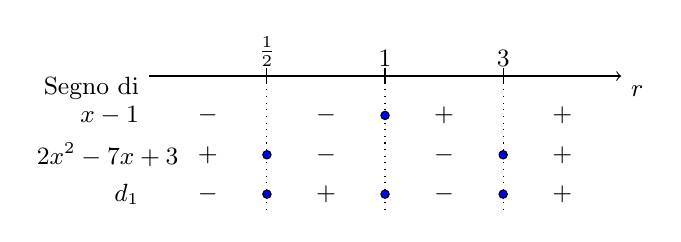
\begin{tikzpicture}[font=\small,x=10mm, y=10mm]

\draw[->] (0,0) -- (6,0) node [below right] () {$r$};

\foreach \x in {1.5,3,4.5}{
\draw(\x,3pt)--(\x,-3pt);
\begin{scope}[dotted]
\draw (\x,0) -- (\x,-1.7);
\end{scope}}

\node[left] at (0,-0.15) {Segno di};
\node[left] at (0,-0.5) {$x-1$};
\node[left] at (.5,-1) {$2x^2-7x+3$};
\node[left] at (0,-1.5) {$d_1$};
\node[above]  at (1.5,0) {$\frac{1}{2}$};
\node[above]  at (3,0) {$1$};
\node[above]  at (4.5,0) {$3$};
\node[] at (.75,-0.5) {$-$};
\node[] at (2.25,-0.5) {$-$};
\node[] at (3.75,-0.5) {$+$};
\node[] at (5.25,-0.5) {$+$};
\node[] at (.75,-1) {$+$};
\node[] at (2.25,-1) {$-$};
\node[] at (3.75,-1) {$-$};
\node[] at (5.25,-1) {$+$};
\node[] at (.75,-1.5) {$-$};
\node[] at (2.25,-1.5) {$+$};
\node[] at (3.75,-1.5) {$-$};
\node[] at (5.25,-1.5) {$+$};

\draw[fill=blue] (3,-.5)circle (1.5pt);
\draw[fill=blue] (1.5,-1)circle (1.5pt);
\draw[fill=blue] (4.5,-1)circle (1.5pt);
\draw[fill=blue] (3,-1.5)circle (1.5pt);
\draw[fill=blue] (1.5,-1.5)circle (1.5pt);
\draw[fill=blue] (4.5,-1.5)circle (1.5pt);

\end{tikzpicture}

% \end{center}
% La disequazione è verificata negli intervalli dove è presente il
% segno ``\(+\)''.
% \[\IS=\left\{x\in\insR/x<\frac{4}{5}\vee~3<x<\frac{9}{2}\right\}.\]
% \end{esempio}
% 
% \begin{esempio}
%  \(4x^{3}+4x^{2}\le~1+x.\)
% La disequazione è di terzo grado; trasportiamo al primo membro tutti i
% monomi:
% \[4x^{3}+4x^{2}-1-x\le~0.\]
% 
% Possiamo risolverla se riusciamo a scomporre in fattori di primo grado
% il polinomio al primo membro:
% \[4x^{3}+4x^{2}-1-x=4x^{2}(x+1)-(x+1)=(x+1)(4x^2-1) \Rightarrow 
% (x+1)(2x-1)(2x+1)\le~0.\]
% 
% Studiamo ora il segno di ciascun fattore, tenendo conto che sono
% richiesti anche i valori che annullano ogni singolo fattore (legge di
% annullamento del prodotto):
% 
% \[ F_{1}:x+1\ge~0\Rightarrow x\ge -1;\quad F_{2}:2x-1\ge~0\Rightarrow x\ge 
% \dfrac{1}{2},\quad F_{3}:2x+1\ge~0\Rightarrow x\ge -{\dfrac{1}{2}}.\]
% Possiamo ora costruire la tabella dei segni.
% Ricordiamo che la disequazione di partenza~\(4x^{3}+4x^{2}\le~1+x\) è
% verificata dove compare il segno~``\(-\)'':
% 
% \begin{center}
% % (c) 2013 Claudio Carboncini - claudio.carboncini@gmail.com
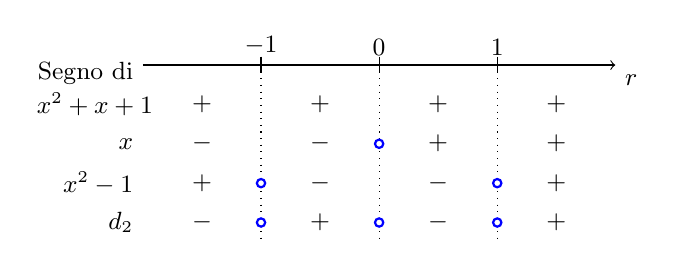
\begin{tikzpicture}[font=\small,x=10mm, y=10mm]

\draw[->] (0,0) -- (6,0) node [below right] () {$r$};

\foreach \x in {1.5,3,4.5}{
\draw(\x,3pt)--(\x,-3pt);
\begin{scope}[dotted]
\draw (\x,0) -- (\x,-2.2);
\end{scope}}

\node[left] at (0,-0.1) {Segno di};
\node[left] at (.25,-0.5) {$x^2+x+1$};
\node[left] at (0,-1) {$x$};
\node[left] at (0,-1.5) {$x^2-1$};
\node[left] at (0,-2) {$d_2$};
\node[above]  at (1.5,0) {$-1$};
\node[above]  at (3,0) {$0$};
\node[above]  at (4.5,0) {$1$};
\node[] at (.75,-0.5) {$+$};
\node[] at (2.25,-0.5) {$+$};
\node[] at (3.75,-0.5) {$+$};
\node[] at (5.25,-0.5) {$+$};
\node[] at (.75,-1) {$-$};
\node[] at (2.25,-1) {$-$};
\node[] at (3.75,-1) {$+$};
\node[] at (5.25,-1) {$+$};
\node[] at (.75,-1.5) {$+$};
\node[] at (2.25,-1.5) {$-$};
\node[] at (3.75,-1.5) {$-$};
\node[] at (5.25,-1.5) {$+$};
\node[] at (.75,-2) {$-$};
\node[] at (2.25,-2) {$+$};
\node[] at (3.75,-2) {$-$};
\node[] at (5.25,-2) {$+$};

\begin{scope}[blue,thick]
\draw[fill=white] (3,-1)circle (1.5pt);
\draw[fill=white] (1.5,-1.5)circle (1.5pt);
\draw[fill=white] (4.5,-1.5)circle (1.5pt);
\draw[fill=white] (3,-2)circle (1.5pt);
\draw[fill=white] (1.5,-2)circle (1.5pt);
\draw[fill=white] (4.5,-2)circle (1.5pt);
\end{scope}

\end{tikzpicture}

% \end{center}
% \[\IS=\left\{x\in \insR/x\le-1\text{ oppure }-\frac{1}{2}\le 
% x\le\frac{1}{2}\right\}.\]
% \end{esempio}
% % \end{exrig}
% 
% \begin{procedura}
%  Determinare l'\(\IS\) Di una disequazione polinomiale di grado
% superiore al primo:
% 
% \begin{enumeratea}
%  \item scrivere la disequazione nella forma~\(p\leq0\), \(p\geq~0\),
% \(p<0\), \(p>0\);
% \item scomporre in fattori irriducibili il polinomio;
% \item determinare il segno di ciascun fattore, ponendolo sempre maggiore
% di zero, o maggiore uguale a zero a seconda della richiesta del
% problema;
% \item costruire la tabella dei segni, segnando con un punto ingrossato
% gli zeri del polinomio;
% \item determinare gli intervalli in cui il polinomio assume il segno
% richiesto.
% \end{enumeratea}
% \end{procedura}
% 
% % \ovalbox{\risolvii \ref{ese:21.44}, \ref{ese:21.45}, \ref{ese:21.46}, 
% \ref{ese:21.47}, \ref{ese:21.48}, \ref{ese:21.49}, \ref{ese:21.50}, 
% \ref{ese:21.51},
% % \ref{ese:21.52}, \ref{ese:21.53}}

% \section{Disequazioni frazionarie}
% \label{sec:21_frazionarie}

% Un'espressione contenente operazioni tra frazioni
% algebriche ha come risultato una frazione algebrica. Con la condizione
% di esistenza che il denominatore della frazione sia diverso da zero la
% ricerca del segno di una frazione algebrica viene effettuata con la
% stessa procedura seguita per il prodotto di due o più fattori.
% 
% % \begin{exrig}
%  \begin{esempio}
%  \(p=\dfrac{3x-7}{2-x}\ge~0\).
% 
%  Poniamo innanzi tutto la~\(\CE: 2-x\neq~0\)
%  cioè~\(x\neq~2\) e procediamo studiando il segno del
% numeratore e del denominatore. Terremo conto della~\(\CE\) ponendo il
% denominatore semplicemente maggiore di zero e non maggiore uguale.
% \[N\ge~0\Rightarrow~3x-7\ge~0\Rightarrow x\ge \frac{7}{3},\]
% \[D>0\Rightarrow2-x>0\Rightarrow \ x<2.\]
% \begin{center}
% % (c) 2012 Dimitrios Vrettos - d.vrettos@gmail.com
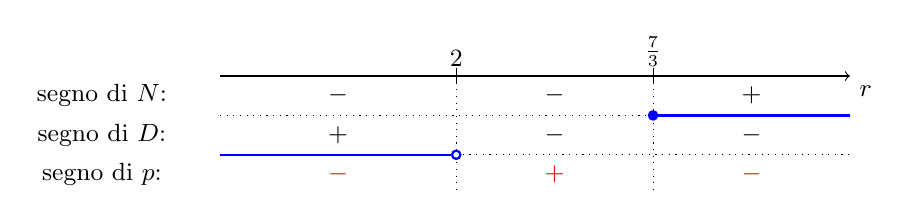
\begin{tikzpicture}[font=\small,x=10mm, y=10mm]

\draw[->] (0,0) -- (8,0) node [below right] () {$r$};

\foreach \x in {3,5.5}{
\draw(\x,3pt)--(\x,-3pt);
\begin{scope}[dotted]
\draw (\x,0) -- (\x,-1.5);
\draw (0,-.5) -- (5.5,-.5);
\draw (3,-1) -- (8,-1);
\end{scope}}

\node[above]  at (3,0) {$2$};
\node[above]  at (5.5,0) {$\frac{7}{3}$};

\begin{scope}[blue,thick]
\draw (5.5,-.5) -- (8,-.5);
\draw (3,-1) -- (0,-1);

\draw[fill=blue] (5.5,-.5)circle (1.5pt);
\draw[fill=white] (3,-1)circle (1.5pt);
\end{scope}

\foreach \x in {-1.5}{
\node  at (\x,-.25) {segno di $N$:};
\node  at (\x,-.75) {segno di $D$:};
\node  at (\x,-1.25) {segno di $p$:};
}
\foreach \z in {1.5,4.25}
\node  at (\z,-.25) {$-$};

\foreach \zi in {4.25,6.75}
\node  at (\zi,-.75) {$-$};

\node  at (6.75,-.25) {$+$};
\node  at (1.5,-.75) {$+$};

\begin{scope}[red]
\foreach \y in {-1.25}{
\foreach \ziv in {4.25}
	\node at (\ziv,\y) {$+$};
\foreach \zv in {1.5,6.75}
\node at (\zv,\y) {$-$};
}
\end{scope}
\end{tikzpicture}
% \end{center}
% Analogamente a quanto fatto per il prodotto, dalla tabella dei segni otteniamo
% \[\IS=\left\{x\in \insR/2<x\le \frac{7}{3}\right\}\]
% in cui vediamo già compresa la~\(\CE\) che inizialmente avevamo posto.
%  \end{esempio}
% % \end{exrig}
% 
% \begin{procedura}
%  Procedura per determinare~\(\IS\) di una disequazione frazionaria:
% 
% \begin{enumeratea}
% \item applicare il primo principio e trasportare tutti i termini al primo 
% membro;
%  \item eseguire i calcoli dell'espressione al primo membro per arrivare a una 
% disequazione nella forma:
%  \subitem \(\dfrac{N(x)}{D(x)}>0\) oppure~\(\dfrac{N(x)}{D(x)}\ge~0\) 
% oppure~\(\dfrac{N(x)}{D(x)}<0\) oppure~\(\dfrac{N(x)}{D(x)}\le~0\);
%  \item studiare il segno del numeratore e del denominatore, ponendo~\(N(x)>0\) 
% (oppure~\(N(x)\geq~0\) a secondo della richiesta) e~\(D(x)>0\);
%  \item costruire la tabella dei segni, segnando con un punto in grassetto gli 
% zeri del numeratore;
%  \item determinare gli intervalli in cui il polinomio assume il segno 
% richiesto.
% \end{enumeratea}
% \end{procedura}
% 
% % \begin{exrig}
%  \begin{esempio}
%  
% \(\dfrac{x-1}{2x+2}+\dfrac{2x+1}{4x-2}>\dfrac{4x^{2}(2x+1)+1}{8x^{3}+8x^{2}-2x-2}
% .\)
% 
% Trasportiamo tutti i termini al primo 
% membro~\(\dfrac{x-1}{2x+2}+\dfrac{2x+1}{4x-2}-\dfrac{4x^{2}(2x+1)+1}{8x^{3}+8x^{2
% }-2x-2}>0\).
% 
% Scomponiamo in fattori i denominatori, determiniamo il minimo comune
% multiplo e sommiamo le frazioni per arrivare alla forma~\(\frac{N(x)}{D(x)}>0\):
% 
% \begin{align}
% 
% &\frac{x-1}{2(x+1)}+\frac{2x+1}{2(2x-1)}-\frac{4x^{2}(2x+1)+1}{
% 2(x+1)(2x-1)(2x+1)}>0 \notag\\
% \Rightarrow & 
% \frac{(x-1)(2x-1)(2x+1)+(2x+1)(2x+1)(x+1)-4x^{2}(2x+1)+1}{2(x+1)(2x-1)(2x+1)}>0 
% \notag\\
% \Rightarrow & \frac{4x+1}{2(x+1)(2x-1)(2x+1)}>0. \label{eq:21.1}
% \end{align}
% Studiamo separatamente il segno di tutti i fattori che compaiono nella
% frazione, sia quelli al numeratore sia quelli al denominatore e
% costruiamo la tabella dei segni:
%  \[\begin{gathered}
%  N>0\Rightarrow~4x+1>0\Rightarrow x>-{\frac{1}{4}},\\
%  D>0\Rightarrow\left\{\begin{array}{l}
% 	\t\tx+1>0\Rightarrow x>-1 \\
% 	\t\t2x-1>0\Rightarrow x>\frac{1}{2}\\
% 	\t\t2x+1>0\Rightarrow x>-{\frac{1}{2}}
% \t	  \end{array}\right..
% \end{gathered}\]
% \begin{center}
% % (c) 2012 Dimitrios Vrettos - d.vrettos@gmail.com
\begin{tikzpicture}[font=\small,x=10mm, y=10mm]

  \draw[->] (0,0) -- (8,0) node [below right] () {$r$};

  \foreach \x in {1.5,2.75,3.75,5.75}{
    \draw(\x,3pt)--(\x,-3pt);
    
    \begin{scope}[dotted]
      \draw (\x,0) -- (\x,-2.5);
      \draw (0,-.5) -- (3.75,-.5);
      \draw (0,-1) -- (1.5,-1);
      \draw (0,-1.5) -- (5.75,-1.5);
      \draw (0,-2) -- (2.75,-2);
    \end{scope}
  }

  \node[above]  at (1.5,0) {$-1$};
  \node[above] at (2.75,0) {$-\frac{1}{2}$};
  \node[above]  at (3.75,0) {$-\frac{1}{4}$};
  \node[above]  at (5.75,0) {$\frac{1}{2}$};

  \begin{scope}[blue,thick]
    \draw (3.75,-.5) -- (8,-.5);
    \draw (1.5,-1) -- (8,-1);
    \draw (5.75,-1.5) -- (8,-1.5);
    \draw (2.75,-2) -- (8,-2);

    \draw[fill=white] (3.75,-.5)circle (1.5pt);
    \draw[fill=white] (1.5,-1)circle (1.5pt);
    \draw[fill=white] (5.75,-1.5)circle (1.5pt);
    \draw[fill=white] (2.75,-2)circle (1.5pt);
  \end{scope}

  \foreach \x in {-1.5}{
    \node  at (\x,-.25) {segno di $N$:};
    \node(d1)  at (\x,-.75) {segno di $d_1$:};
    \node  at (\x,-1.25) {segno di $d_2$:};
    \node (d3) at (\x,-1.75) {segno di $d_3$:};
    \node  at (\x,-2.25) {segno di $f$:};
    }

  \draw[decorate, decoration={brace, mirror}] let \p1=(d1.north west), \p2=(d3.south west) in(\p1 ) -- (\p2) node[midway, left=2pt] {$D:$};

  \foreach \z in {.75, 2.125,3.25}
    \node  at (\z,-.25) {$-$};

  \foreach \zi in {4.75, 6.875}
    \node  at (\zi,-.25) {$+$};

  \foreach \zii in {2.125,3.25,4.75, 6.875}
    \node  at (\zii,-.75) {$+$};

  \foreach \ziii in {.75,2.125,3.25,4.75}
    \node  at (\ziii,-1.25) {$-$};

  \foreach \ziv in {.75,2.125}
    \node at (\ziv,-1.75) {$-$};

  \foreach \zv in {3.25,4.75, 6.875}
    \node at (\zv,-1.75) {$+$};

  \node  at (.75,-.75) {$-$};
  \node  at (6.875,-1.25) {$+$};

  \begin{scope}[red]
    \foreach \y in {-2.25}{
      \foreach \ziv in {.75,3.25,6.875}
	\node at (\ziv,\y) {$+$};
      \foreach \zv in {2.125,4.75}
	\node at (\zv,\y) {$-$};
    }
  \end{scope}
\end{tikzpicture}
% \end{center}
% Non abbiamo posto le~\(\CE\) in quanto già rispettate dalle disequazioni
% del denominatore.
% Prendiamo gli intervalli in cui il segno della frazione è positivo
% come richiesto dalla disequazione~\ref{eq:21.1}:
%  \[\IS=\left\{x\in \insR/x<-1\vee -{\frac{1}{2}}<x<-{\frac{1}{4}}\vee 
% x>\frac{1}{2}\right\}.\]
% \end{esempio}
% 
%  \begin{esempio}
% \(\dfrac{x}{2}-\dfrac{2}{3}\cdot 
% {\dfrac{2x-3}{x-1}}+\dfrac{10x-3}{6x-6}\le\dfrac{3}{2}\cdot 
% {\dfrac{x^{2}+2}{3x-2}}+\dfrac{1}{3(x-1)(3x-2)}.\)
% 
% Trasportiamo tutti i termini al primo membro:
% 
% \[\frac{x}{2}-\frac{2}{3}\cdot\frac{2x-3}{x-1}+\frac{10x-3}{6x-6}-\frac{3}{2}
% \cdot\frac{x^{2}+2}{3x-2}-\frac{1}{3(x-1)(3x-2)}\le~0.\]
% 
% Eseguiamo le operazioni per semplificare la frazione e ridurla alla
% forma~\(\frac{N(x)}{D(x)}\le~0\):
% 
% \begin{align}
%   
% &\frac{x}{2}-\frac{4x-6}{3(x-1)}+\frac{10x-3}{6(x-1)}-\frac{3x^{2}+6}{2(3x-2)}
% -\frac{1}{3(x-1)(3x-2)}\le~0\notag\\
%   \Rightarrow 
% &\frac{3x(x-1)(3x-2)-2(4x-6)(3x-2)+(10x-3)(3x-2)-3(3x^{2}+6)(x-1)-2}{
% 6(x-1)(3x-2)}\le~0\notag\\
%   \Rightarrow &\frac{11x-2}{6(x-1)(3x-2)}\le~0. \label{eq:22.2}
% \end{align}
% 
% Studiamo il segno del numeratore e dei fattori del denominatore:
%  \[\begin{gathered}N\ge~0\Rightarrow~11x-2\ge~0\Rightarrow x\ge\frac{2}{11},\\
% \t	  D>0\Rightarrow\left\{\begin{array}{l}
% 	\t\td_{1}>0\Rightarrow x-1>0\Rightarrow x>1\\
% 	\t\td_{2}>0\Rightarrow~3x-2>0\Rightarrow x>\dfrac{2}{3}
% 	\t	\end{array}\right.. \end{gathered}\]
% \begin{center}
% % (c) 2012 Dimitrios Vrettos - d.vrettos@gmail.com
\begin{tikzpicture}[font=\small,x=10mm, y=10mm]

\draw[->] (0,0) -- (8,0) node [below right] () {$r$};

\foreach \x in {1,3.72,5.56}{
\draw(\x,3pt)--(\x,-3pt);
\begin{scope}[dotted]
\draw (\x,0) -- (\x,-2);
\draw (0,-.5) -- (1,-.5);
\draw (0,-1) -- (5.56,-1);
\draw (0,-1.5) -- (3.72,-1.5);

\end{scope}}


\node[above] at (1,0) {$\frac{2}{11}$};
\node[above]  at (3.72,0) {$\frac{2}{3}$};
\node[above]  at (5.56,0) {$1$};

\begin{scope}[blue,thick]
\draw (1,-.5) -- (8,-.5);
\draw (5.56,-1) -- (8,-1);
\draw (3.72,-1.5) -- (8,-1.5);

\draw[fill=blue] (1,-.5)circle (1.5pt);
\draw[fill=white] (5.56,-1)circle (1.5pt);
\draw[fill=white] (3.72,-1.5)circle (1.5pt);
\end{scope}

\foreach \x in {-1.5}{
\node  at (\x,-.25) {segno di $N$:};
\node(d1)  at (\x,-.75) {segno di $d_1$:};
\node (d2) at (\x,-1.25) {segno di $d_2$:};
\node (d3) at (\x,-1.75) {segno di $f$:};
}

 \draw[decorate, decoration={brace, mirror}]  let \p1=(d1.north west), \p2=(d2.south west) in(\p1 ) -- (\p2) node[midway, left=2pt] {$D:$};

\foreach \z in {2.36,4.64,6.78}
\node  at (\z,-.25) {$+$};

 \foreach \zi in {.5,2.36,4.64}
 \node  at (\zi,-.75) {$-$};

\foreach \zii in {.5,2.36}
 \node  at (\zii,-1.25) {$-$};

 \foreach \ziii in {4.64,6.78}
\node  at (\ziii,-1.25) {$+$};

\node  at (.5,-.25) {$-$};
\node  at (6.78,-.75) {$+$};

\begin{scope}[red]
\foreach \y in {-1.75}{
\foreach \ziv in {.5,4.64}
	\node at (\ziv,\y) {$-$};
\foreach \zv in {2.36,6.78}
\node at (\zv,\y) {$+$};
}
\end{scope}
\end{tikzpicture}
% \end{center}
% Non abbiamo posto le~\(\CE\) in quanto già rispettate dalle disequazioni
% del denominatore. Prendiamo gli intervalli in cui il segno della frazione è 
% positivo o
% nullo come dalla disequazione~\ref{eq:22.2}:
% \[\IS=\left\{x\in \insR/x\le\frac{2}{11}\vee \frac{2}{3}<x<1\right\}.\]
%  \end{esempio}
% % \end{exrig}
% % \ovalbox{\risolvii \ref{ese:21.54}, \ref{ese:21.55}, \ref{ese:21.56}, 
% \ref{ese:21.57}, \ref{ese:21.58}, \ref{ese:21.59}, \ref{ese:21.60}, 
% \ref{ese:21.61}, \ref{ese:21.62}, \ref{ese:21.63}}
% 
% % \vspazio\ovalbox{\ref{ese:21.64}, \ref{ese:21.65}, \ref{ese:21.66}, 
% \ref{ese:21.67}, \ref{ese:21.68}, \ref{ese:21.69}}
